\documentclass[a4paper, 8pt]{extarticle}

% ------------------------------------------------------------------
% Imports
% ------------------------------------------------------------------

% Formatting
\usepackage[landscape, left=.5cm, top=.5cm, right=.5cm, bottom=.5cm]{geometry}
\usepackage{flowfram}
\usepackage[compact]{titlesec}
\usepackage{parskip}
\usepackage{mathptmx} % times font

% Language stuff
\usepackage[english]{babel}
\usepackage[utf8]{inputenc}

% Math imports
\usepackage{amsthm}
\usepackage{amssymb}
\usepackage{amsmath}
\usepackage{bm}
\usepackage{mathtools}

% Tables
\usepackage{tabularx} % tabularx since the width should be handled automatically
\usepackage{makecell}
\usepackage{multirow}

% Graphics
\usepackage{graphics}

% Miscellaneous
\usepackage{hyperref}
\usepackage{enumerate}
\usepackage[inline]{enumitem}
\usepackage{multicol}
\usepackage{xcolor}
\usepackage{etoolbox}
\usepackage{mdframed}
\usepackage{listings}
\usepackage{algpseudocode}
\makeatletter
\DeclareDocumentCommand{\mdtheorem}{ O{} m o m o }%
 {\ifcsdef{#2}%
   {\mdf@PackageWarning{Environment #2 already exits\MessageBreak}}%
   {%
    \IfNoValueTF {#3}%
     {%#3 not given -- number relationship
      \IfNoValueTF {#5}%
        {%#3+#5 not given
        \@definecounter{#2}%
        \expandafter\xdef\csname the#2\endcsname{\@thmcounter{#2}}%
        \newenvironment{#2}[1][]{%
          \refstepcounter{#2}%
          \ifstrempty{##1}%
            {\let\@temptitle\relax}%
            {%
             \def\@temptitle{\mdf@theoremseparator%
                             \mdf@theoremspace%
                             \mdf@theoremtitlefont%
                             ##1}%
             \mdf@thm@caption{#2}{{#4}{\csname the#2\endcsname}{##1}}%
             }%
          \begin{mdframed}[#1,frametitle={\strut#4\ \csname the#2\endcsname%
                                          \@temptitle}]}%
          {\end{mdframed}}%
        \newenvironment{#2*}[1][]{%
          \ifstrempty{##1}{\let\@temptitle\relax}{\def\@temptitle{\mdf@theoremseparator \mdf@theoremspace ##1}}% <- the problem was here
          \begin{mdframed}[#1,frametitle={\strut#4\@temptitle}]}%
          {\end{mdframed}}%
        }%
        {%#5 given -- reset counter
        \@definecounter{#2}\@newctr{#2}[#5]%
        \expandafter\xdef\csname the#2\endcsname{\@thmcounter{#2}}%
        \expandafter\xdef\csname the#2\endcsname{%
               \expandafter\noexpand\csname the#5\endcsname \@thmcountersep%
                  \@thmcounter{#2}}%
        \newenvironment{#2}[1][]{%
          \refstepcounter{#2}%
          \ifstrempty{##1}%
            {\let\@temptitle\relax}%
            {%
             \def\@temptitle{\mdf@theoremseparator%
                             \mdf@theoremspace%
                             \mdf@theoremtitlefont%
                             ##1}%
             \mdf@thm@caption{#2}{{#4}{\csname the#2\endcsname}{##1}}%
             }
          \begin{mdframed}[#1,frametitle={\strut#4\ \csname the#2\endcsname%
                                          \@temptitle}]}%
          {\end{mdframed}}%
        \newenvironment{#2*}[1][]{%
          \ifstrempty{##1}%
            {\let\@temptitle\relax}%
            {%
             \def\@temptitle{\mdf@theoremseparator%
                             \mdf@theoremspace%
                             \mdf@theoremtitlefont%
                             ##1}%
             \mdf@thm@caption{#2}{{#4}{\csname the#2\endcsname}{##1}}%
             }%
          \begin{mdframed}[#1,frametitle={\strut#4\@temptitle}]}%
          {\end{mdframed}}%
        }%
     }%
     {%#3 given -- number relationship
        \global\@namedef{the#2}{\@nameuse{the#3}}%
        \newenvironment{#2}[1][]{%
          \refstepcounter{#3}%
          \ifstrempty{##1}%
            {\let\@temptitle\relax}%
            {%
             \def\@temptitle{\mdf@theoremseparator%
                             \mdf@theoremspace%
                             \mdf@theoremtitlefont%
                             ##1}%
             \mdf@thm@caption{#2}{{#4}{\csname the#2\endcsname}{##1}}%
             }
          \begin{mdframed}[#1,frametitle={\strut#4\ \csname the#2\endcsname%
                                          \@temptitle}]}%
          {\end{mdframed}}%
        \newenvironment{#2*}[1][]{%
          \ifstrempty{##1}{\let\@temptitle\relax}{\def\@temptitle{:\ ##1}}%
          \begin{mdframed}[#1,frametitle={\strut#4\@temptitle}]}%
          {\end{mdframed}}%
     }%
   }%
 }
\makeatother
\usepackage{tikz}
\usetikzlibrary{positioning, shapes.multipart, fit}

% ------------------------------------------------------------------
% Formatting
% ------------------------------------------------------------------

% Colors
\definecolor{accent}{HTML}{272744}
\definecolor{H1}{HTML}{8b6d9c}
\definecolor{H2}{HTML}{f2d3ab}
\definecolor{H3}{HTML}{494d7e}

% Column format
\setlength{\columnsep}{5pt}
\ffvadjustfalse
\Ncolumn{4}
\setlength{\parindent}{0pt}
\setlength{\parskip}{0cm}

% Compact titles
\newcommand{\colorsection}[2]{\colorbox{#1}{\parbox{\dimexpr\linewidth-2\fboxsep}{\centering\ #2}}}
\titlespacing{\section}{0pt}{0pt}{0pt}
\titleformat{\section}{\bfseries\color{white}}{}{0pt}{\colorsection{accent}}

\titlespacing{\subsection}{0pt}{0pt}{0pt}
\titleformat{\subsection}{\bfseries\color{white}}{}{0pt}{\colorsection{accent!60}}

% Compact math mode
\makeatletter
\g@addto@macro\normalsize{%
  \setlength{\abovedisplayskip}{0pt}
  \setlength{\belowdisplayskip}{0pt}
  \setlength{\abovedisplayshortskip}{0pt}
  \setlength{\belowdisplayshortskip}{0pt}
  \setlength{\jot}{0pt}
}
\let\displaystyle\textstyle
\makeatother

% Set each display in math mode to be rendered as \textstyle
\renewcommand{\[}{\phantom{}\begin{center}\(}
\renewcommand{\]}{\)\end{center}}


% Misc
\hypersetup{colorlinks=true, urlcolor=accent, linkcolor=accent, citecolor=accent}
\setlist{itemsep=0.2pt, topsep=0.5pt, leftmargin=5mm}
\renewcommand{\labelenumii}{\arabic{enumi}.\arabic{enumii}}


% definition environments
\newtheoremstyle{compact_theorem}{}{}{\color{H3}\normalfont}{}{\bfseries}{}{0em}{Thm. }
\theoremstyle{compact_theorem}
\newtheorem*{theorem}{Theorem}
\newtheoremstyle{compact_theorems}{}{}{\color{H3}\normalfont}{}{\bfseries}{}{0em}{Thms. }
\theoremstyle{compact_theorems}
\newtheorem*{theorems}{Theorems}
\newtheoremstyle{compact_definition}{}{}{\normalfont}{}{\bfseries}{}{0em}{\thmnote{#3}: }
\theoremstyle{compact_definition}
\newtheorem*{definition}{Definition}

% Colored boxes for algorithms
\mdfdefinestyle{mdalgorithm}{
  hidealllines=true,
  innertopmargin=2pt,
  innerbottommargin=2pt,
  innerrightmargin=2pt,
  innerleftmargin=2pt,
  leftmargin=0pt,
  rightmargin=0pt,
  frametitleaboveskip=2pt,
  frametitlebelowskip=2pt,
  theoremseparator={},
  theoremspace={},
  skipabove=2pt,
  skipbelow=2pt,
  backgroundcolor=H1!30,
}

\newenvironment{algorithm}%
    {\begin{mdframed}[style=mdalgorithm]\begin{definition}}%
    {\end{definition}\end{mdframed}}


% ------------------------------------------------------------------
% Custom Commands
% ------------------------------------------------------------------

% Math general
\DeclareMathOperator{\R}{\mathbb{R}}
\DeclareMathOperator{\N}{\mathbb{N}}
\DeclareMathOperator{\Z}{\mathbb{Z}}
\DeclareMathOperator{\C}{\mathbb{C}}
\renewcommand{\O}{\mathcal{O}}
\renewcommand{\P}{\mathbb{P}}
\renewcommand{\Im}{\text{Im}}
\DeclareMathOperator{\E}{\mathbb{E}}
\DeclareMathOperator{\F}{\mathcal{F}}
\renewcommand{\L}{\mathcal{L}}
\DeclareMathOperator{\Var}{\mathbb{V}}
\DeclareMathOperator{\Cov}{Cov}
\DeclareMathOperator{\argmin}{argmin}
\DeclareMathOperator{\argmax}{argmax}
\DeclareMathOperator{\I}{\mathbb{I}}
\DeclareMathOperator{\margin}{margin}
\DeclareMathOperator{\normal}{\mathcal{N}}
\DeclareMathOperator{\unif}{\mathcal{U}}
\DeclareMathOperator{\cat}{Cat}
\DeclareMathOperator{\tr}{Tr}

% Misc
\newcommand{\sdots}{\ifmmode\mathinner{\ldotp\kern-0.2em\ldotp\kern-0.2em\ldotp}\else.\kern-0.13em.\kern-0.13em.\fi}


% ------------------------
% Document
% ------------------------

\begin{document}

% Title
% \begin{center}
%   \large Introduction to ML \\
%   \small \(\langle\)\href{https://google.com}{nicstuder@student.ethz.ch}\(\rangle\)
% \end{center}

% Visual computing
\section{The Digital Image}

\begin{definition}[Problems]
   Transmission inference, artifacts, scratches, noise, bad contrast / resolution, motion blur, spilling
\end{definition}

\begin{definition}[Image]
  Pattern of a value varying in space and/or time.
\end{definition}

\begin{definition}[Pixel]
  Discrete samples of a continuous image function.
\end{definition}

\subsection{Sensors}
\begin{definition}[Charge Coupled Device (CCD)]
  Contains sensor array (array of photosites [bucket of electrical charge]), ADC (digitalize measurement line by line) and image array. \textit{Sequential} readout.
  \begin{itemize}[label=-]
    \item \textbf{Blooming}: Oversaturation of photosites \(\implies\) flooding.
    \item \textbf{Bleeding/Smearing}: Accumulate charges during readout.
    \item \textbf{Dark Current}: Thermally generated charge \(\Rightarrow\) non-0 output. Reduced by cooling or avg. dark images and subtract.
  \end{itemize}
\end{definition}

\begin{definition}[CMOS]
  Same sensor as CCD, but with amplifiers.
  \begin{itemize*}
    \item cheaper
    \item lower power
    \item less sensitive
    \item per pixel amplification
    \item random pixel access
    \item no blooming
    \item on chip integration
  \end{itemize*}

  For videos: rolling shutter due to sequential read-out of lines.
\end{definition}

\begin{definition}[Dynamic Vision Sensor (DVS)]
  Smart pixels: ind. and async.
\end{definition}

\subsection{Sampling and Quantization}
\begin{definition}[Sampling]
  \begin{itemize*}
    \item Cartesian (grid)
    \item Hexagonal
    \item non-uniform
  \end{itemize*}

  Reconstruction with e.g. bilinear interpolation.
\end{definition}

\begin{definition}[Quantization]
  \(\R \to \Z\), lossy, simple quant. with \(k = 2^b\) levels.
\end{definition}

\begin{definition}[Resolutions]
  \begin{itemize*}
    \item \textit{Image}: px \(\times\) px
    \item \textit{Geometric}: \#pixels per area
    \item \textit{Radiometric}: \#bits per pixel
  \end{itemize*}
\end{definition}

\begin{definition}[Additive Gaussian Noise]
  \(I(x, y) = f(x, y) + c, \ c \sim \normal(0, \sigma^2)\)
\end{definition}

\begin{definition}[Poisson Noise]
  Shot noise for low light as \(\normal\) can be \(< 0\).
\end{definition}

\begin{definition}[Quantization Error]
  \(c \sim \unif([-0.5, 0.5], [-0.5, 0.5])\)
\end{definition}

\begin{definition}[Rician noise]
  Noise that appears in MRI.
\end{definition}

\begin{definition}[SNR]
  Index of quality: \(s = \frac{F}{\sigma}, \quad F = \frac{1}{XY}\sum_{x=1}^X\sum_{y=1}^Y f(x, y)\). \textit{PSNR} (Peak SNR) \(s_\text{peak} = \frac{F_{\max}}{\sigma}\) often used in practice.
\end{definition}

\subsection{Color Cameras}
\begin{definition}[Prism]
  Separate light in 3 beams to 3 sensors.
\end{definition}

\begin{definition}[Filter Mosaic]
  Coat rasterized filter (filter out different colors).
\end{definition}

\begin{definition}[Filter Wheel]
  Rotate multiple filters in front of lens.
\end{definition}

\begin{definition}[CMOS]
  Absorb colors at different depths \(\implies\) better quality.
\end{definition}

\begin{tabularx}{\linewidth}{|X|X|X|X|}
  \hline
  Approach & Prism & Mosaic & Wheel \\ \hline
  \# Sensors & 3 & 1 & 1 \\ \hline
  Separation & High & Avg. & Good \\ \hline
  Cost & High & Low & Average \\ \hline
  Framerate & High & High & Low \\ \hline
  Artifacts & Low & Aliasing & Motion \\ \hline
  Bands & 3 & 3 & \(\geq 3\) \\ \hline
  Usage & High-End & Low-end & Scientific \\ \hline
\end{tabularx}

\section{Image Segmentation}
\begin{definition}[Complete Segmentation]
  \(I = \bigcup_{i=1}^N R_i \land \forall i \neq j. R_i \cap R_j = \emptyset\)
\end{definition}

\subsection{Thresholding}

\begin{definition}[Thresholding]
  Produce binary image \(B\) with in/out pixels.
  \[B(x, y) = 1  \iff I(x, y) \geq \tau\]
  Find \(\tau\) with ROC Analysis or greylevel histogram. Use surface coherence from the image context to improve result.
\end{definition}

\begin{definition}[Chromakeying]
  Use BG color: \(B(x, y) = |I(x, y) - c_{BG}| > \tau\).
  Problem: variation due to lighting, noise, etc.
  Thus normalize the color per pixel: \(c = (\frac{R}{I}, \frac{G}{I}, \frac{B}{I}), \quad I = R + G + B\).
\end{definition}

\begin{definition}[Receiver Operating Characteristic (ROC) Analysis]
  Find good \(\tau\) by plotting \(\text{TPR} = \frac{\text{TP}}{\text{TP} + \text{FN}}\) against \(\text{FPR} = \frac{\text{FP}}{\text{TN} + \text{FP}}\) for different \(\tau\). 
  Choose point with gradient \(\beta = \frac{N}{P} \frac{V_{TN} + C_{FP}}{V_{TP} + C_{FN}}\).
\end{definition}

\subsection{Pixel Connectivity}
Either 4- or 8-connectivity. A region is \(x\)-connected, if every pair of pixels contains a \(x\)-connected pixel path.

\begin{definition}[Region Growing]
  Start from \textit{seed point}. Add neighboring pixels that satisfy the inclusion criteria, repeat until fixed.

  \begin{itemize}
    \item \textbf{Seed region}: by hand or conservative thresholding
    \item \textbf{Inclusion criteria}: greylevel thresholding, greylevel distribution model (include if \((I(x, y) - \mu^2)^2 < (n \sigma)^2\) and update \(\mu, \sigma\) after each iteration)
    \item \textbf{Snakes}: Active contour (polygon) where each point moves away from seed while criteria is met.
    Available \textit{smoothness} constraints.
    Iteratively minimize the energy function \(E = E_{\text{tension}} + E_{\text{stiffness}} + E_{\text{image}}\).
  \end{itemize}
\end{definition}

\subsection{Foreground-Background Segmentation}
Need info about the BG \(I_{bg}\). Can be a color or even an image!
\begin{itemize}
  \item \textit{Simple distance measurement}: \(I_\alpha = |I - I_{bg}| < \tau\).
  \item \textit{Mahalanobis distance}: \(I_\alpha = \sqrt{(I - I_{bg})^\top \Sigma^{-1}(I - I_{bg})}\) with emp. cov. \(\Sigma = \frac{1}{n - 1} \sum_{i=1}^n (x_i - \mu) (x_i - \mu)^\top\), \(\mu\) sample mean.
\end{itemize}
Mean and covariance per pixel, but one threshold for all pixels.

\subsection{Morphological operators}
Logical transformations based on comparison of neighboring pixels with a pattern.
\begin{itemize}
  \item \textbf{Erode} \(\ominus\): Erase FG pixel that has a BG neighbor.
  \item \textbf{Dilate} \(\oplus\): Paint BG pixel to FG, if it has a FG neighbor.
  \item \textbf{Opening}: \((I \ominus S) \oplus S \quad \bullet\) \textbf{Closing}: \((I \oplus S) \ominus S\)
\end{itemize}

\section{Image Filtering}
Modify pixels based on linear-combination of neighborhood.
\[I'(x, y) = \sum_{(i, j) \in N(x, y)} K(x, y; i, j)I(i, j)\]

\begin{definition}[Shift-Invariant]
  \(K\) independent of \((x, y) \iff\) same for all px
\end{definition}

\begin{definition}[Separable \(K\)]
  \(K(i, j) = f(i) \cdot g(j) \iff \text{rank}(K) = 1\)
\end{definition}

\begin{definition}[Correlation (\(K \circ I\))]
  Also called \textit{pattern matching}.
  \[I'(x, y) = \sum_{(i, j) \in N(x, y)} K(i, j) I(x + i, y + j)\]
\end{definition}

\begin{definition}[Convolution (\(K \ast I\))]
  Also called \textit{point spread}.
  \begin{align*}
    I'(x, y) &= \sum_{(i, j) \in N(x, y)} K(i, j) I(x - i, y - j) \\
    &= \sum_{(i, j) \in N(x, y)} K(-i, -j) I(x + i, y + j) \\
  (f \ast g)(t) &= \int_{\R} f(t')g(t - t') \, dt' \qquad (\text{cont. case})
  \end{align*}

  \textit{Properties}:
  \begin{itemize*}
    \item Local (only \(N(x, y)\))
    \item Associative
    \item Shift invariant
    \item Linear (\(k \ast (\alpha I_1 + \beta I_2) = \alpha(k \ast I_1) + \beta(k \ast I_2)\))
    \item Commutative
    \item Distributive over +
  \end{itemize*}
\end{definition}

\begin{theorems}
  \begin{itemize*}
    \item \(K(i, j) = K(-i, -j) \implies \circ \equiv \ast\) \\
    \item convolution is correlation with point-mirrored kernel \(K\)
  \end{itemize*}
\end{theorems}

\begin{definition}[Edge Handling]
  \begin{itemize*}
    \item clip filter (black)
    \item wrap around
    \item copy edge
    \item reflect across edge
    \item vary filter near edge
  \end{itemize*}
\end{definition}


\subsection{Special Filters}

\begin{tabularx}{\linewidth}{cc}
  Identity \(\delta\): \(\begin{bmatrix}
    0 & 0 & 0 \\
    0 & 1 & 0 \\
    0 & 0 & 0
  \end{bmatrix}\) & 
  Left Shift (conv.): \(\begin{bmatrix}
    0 & 0 & 0 \\
    1 & 0 & 0 \\
    0 & 0 & 0
  \end{bmatrix}\)
\end{tabularx}

\subsection{Low-Pass Filters (Smoothing)}
Suppress high frequencies (e.g. fine scale details, edges, noise).
Result is equivalent to \textit{smoothing}.

\begin{definition}[Box filter]
  All same values, normalized so sum = 1.
\end{definition}

\begin{definition}[Gaussian Kernel]
  \(G_\sigma = \frac{1}{2 \pi \sigma^2} \exp\left(-\frac{(x^2 + y^2)}{2\sigma^2}\right)\)

  \textit{Properties}:
  \begin{itemize*}
    \item rotationally symmetric
    \item single lobe in both domains
    \item simple relation to \(\sigma\)
    \item efficient
  \end{itemize*}
\end{definition}

\begin{theorem}
  \(G \sim \normal(0, \sigma^2) \implies G \ast G \sim \normal(0, (\sigma \sqrt{2})^2)\)
\end{theorem}

\subsection{High-Pass Filters (Sharpening)}
Suppresses low frequencies which is equivalent to sharpening the edges. Suppressed low frequencies correspond to areas of constant gray level. \textit{Result equivalent to difference between original image and image filtered by Gaussian}.

\begin{definition}[Construction]
  HPF = Identity - LPF
\end{definition}

\begin{theorem}
  Subtracting 1 from centre of LPF, gives negative HPF.
  \((f - \delta) \ast a = f \ast a - \delta \ast a = f \ast a - a = -(a - (f \ast a))\)
\end{theorem}

\begin{definition}[Image Sharpening]
  \(I' = I + \alpha |k \ast I|\), w/ \(k\) HPF and \(\alpha \in [0, 1]\)
\end{definition}

\begin{tabularx}{\linewidth}{cc}
  Laplacian: \(\begin{bmatrix}
    0 & 1 & 0 \\
    1 & -4 & 1 \\
    0 & 1 & 0
  \end{bmatrix}\) & 
  High-pass: \(\begin{bmatrix}
    -1 & -1 & -1 \\
    -1 & 8 & -1 \\
    -1 & -1 & -1
  \end{bmatrix}\)
\end{tabularx}

\subsection{Band Filters}

\begin{definition}[Band pass filter]
  LPF and HPF with cutoffs \(D_{LP} < D_{HP}\)
\end{definition}

\begin{definition}[Band reject filter]
  LPF and HPF with cutoffs \(D_{LP} > D_{HP}\)
\end{definition}

\subsection{Differential Filters}
Edges correspond to points with \textit{high} gradient magnitude. Thus we can approximate the derivative with a simple convolution:
\begin{center}
  \(\frac{\partial f}{\partial x} = \lim_{\epsilon \to 0}\left(\frac{f(x + \epsilon, y) - f(x, y)}{\epsilon}\right) \approx \left(\frac{f(x_{n+1}, y) - f(x_n, y)}{\varDelta x}\right)\)
\end{center}

\begin{definition}[Gradient Magnitude]
  \(M(x, y) = \sqrt{\left(\partial_x f\right)^2 + \left(\partial_y f\right)^2}\)
\end{definition}

\begin{definition}[Gradient Angle]
  \(\alpha(x, y) = \tan^{-1}\left(\partial_y f / \partial_x f\right)\)
\end{definition}

\begin{tabularx}{\linewidth}{cc}
  Prewitt\(_x\): \(\begin{bmatrix}
    -1 & 0 & 1 \\
    -1 & 0 & 1 \\
    -1 & 0 & 1
  \end{bmatrix}\) & 
  Sobel\(_x\): \(\begin{bmatrix}
    -1 & 0 & 1 \\
    -2 & 0 & 2 \\
    -1 & 0 & 1
  \end{bmatrix}\) \\
  \(\frac{\partial I}{\partial x} = \begin{bmatrix}
    -1 & 1
  \end{bmatrix} \ast I\) &
  \(\frac{\partial I}{\partial y} = \begin{bmatrix}
    -1 & 1
  \end{bmatrix}^\top \ast I\)
\end{tabularx}


\section{Image Features}

\subsection{Template Matching}
\textbf{Problem}: Locate an object, described by a template \(t(x, y)\).
{\color{H1}Remove mean before template matching to avoid bias towards bright image areas.}
Two ways to solve the problem:

\begin{definition}[Minimize MSE]
  \(E(p, q) = \sum_{x} \sum_{y}[I(x, y) - t(x - p, y - q)]^2\)
\end{definition}

\begin{definition}[Maximize Area Correlation]
  \(r(p, q) = I(p, q) \ast t(-p, -q)\)
\end{definition}

\subsection{Edge Detection}

\begin{definition}[Edge]
  Local max in 1st \textit{or} zero crossing in 2nd derivative.
\end{definition}

\begin{definition}[Gradient Magnitude]
  \(M(x, y) = \sqrt{\left(\partial_x f\right)^2 + \left(\partial_y f\right)^2}\)
\end{definition}

\begin{definition}[Gradient Angle]
  \(\alpha(x, y) = \tan^{-1}\left(\partial_y f / \partial_x f\right)\)
\end{definition}

\begin{algorithm}[Gradient-Thresholding]
  \begin{enumerate}
    \item Calculate 1st derivative of img
    \item \(B(x, y) = 1 \iff M(x, y) > \tau\)
  \end{enumerate}

  Properties:
  \begin{itemize*}
    \item thick edges
  \end{itemize*}
\end{algorithm}

\begin{definition}[Laplacian operator]
  Detect discontinuities by using second derivatives:
  \(\nabla^2f(x, y) = \partial_{x^2} f(x, y) + \partial_{y^2}f(x, y)\) with discrete approximation kernel \textit{Laplacian} or negative \textit{High-pass}.

  \begin{itemize*}
    \item Isotropic (rotationally invariant)
    \item zero-crossing mark edge locations
    \item sensitive to fine details and noise \(\implies\) blur first
  \end{itemize*}
\end{definition}

\begin{algorithm}[LoG]
  Blur with Gaussian and Laplacian in one convolution:
  \[\text{LoG}(x, y) = -\frac{1}{\pi \sigma^4} \left[1 - \frac{x^2 + y^2}{2\sigma^2}\right]\exp\left(-\frac{x^2 + y^2}{2\sigma^2}\right)\]

  Calculate zero-crossings for edge detection.

  Properties:
  \begin{itemize*}
    \item thin edges
    \item lines are loops
    \item sensitive to noise
  \end{itemize*}
\end{algorithm}

\pagebreak
\begin{algorithm}[Canny]
  \begin{enumerate}
    \item Smooth with Gaussian filter
    \item Compute gradient magnitude and angle
    \item Apply \textbf{non-maxima suppression} to gradient magnitude:
    \textit{Quantize edge normal. If \(M(x, y)\) smaller than neighbor in edge normal direction, drop. Thin multi-pixel ridges.}
    \item \textbf{Hysteresis} with \textbf{Double thresholding} to detect strong and weak edge px's. Partition output into three partitions:
    \begin{center}
      \(\text{no edge} < \tau_{\text{weak}} \leq \text{weak edge} < \tau_{\text{strong}} \leq \text{strong edge}\)
    \end{center}
    Reject weak edge px not connected with strong edge px.
  \end{enumerate}

  Properties:
  \begin{itemize*}
    \item thin edges, edges may be interrupted
  \end{itemize*}
\end{algorithm}

\subsection{Primitive Detection}

\begin{definition}[Parameter Space]
  Space of possible parameter values that define a particular mathematical primitive.
\end{definition}

\begin{definition}[Line Parameterization]
  \begin{enumerate}
    \item \(y = ax + b\): infinite slope, vertical lines cannot be detected. Param space: \(b = -x_i a + y_i\)
    \item \(x \cos \theta + y \cdot \sin \theta = \rho\): Avoids infinite slope.
  \end{enumerate}
\end{definition}

\begin{algorithm}[Hough Transform]
  \begin{enumerate}
    \item Subdivide param space into discrete bins, set bin-count to 0 for all bins.
    \item Draw \textbf{multiple} lines through \((x, y)\) in param space for each edge pixel \((x, y)\) and increment counts along line.
    \item Detect peaks in bins. These are the edge lines.
  \end{enumerate}
\end{algorithm}

\begin{definition}[Hough Transform for circles]
  If \(r\) known: calculate circles with radius \(r\) around edge pixels. Where lots of them meet is the center of a circle. Else we use 3D hough transform with parameters \(x_0, y_0, r\).
\end{definition}

\subsection{Keypoint / Corner Detection}
Edges well localized only in one direction \(\to\) detect corners.
\textit{Desired Properties}:
\begin{itemize*}
  \item accurate localization
  \item Invariance against shift, rotation, scale, brightness change
  \item Robust against noise, high repeatability
\end{itemize*}

\begin{definition}[Local displacement sensitivity]
For patch at point \((x, y)\), it is the MSE intensity change given a displacement vector \(\Delta\).
It can be approximated by \(S(\Delta) = \Delta^\top M \Delta\)
where \(M\) is the normal matrix, given by \(\sum_{(x, y) \in \text{window}} \nabla^2 I(x, y)\).

\end{definition}


\begin{algorithm}[Harris Corner Detection]
  Find points with large \(\min \Delta^\top M \Delta\) for \(||\Delta|| = 1\), which is equivalent to maximize the EVs of \(M\).

  Calculate "cornerness" with \(C(x, y) = \det(M) - k \cdot \tr(M)^2 = \lambda_1 \lambda_2 - k(\lambda_1 + \lambda_2)^2\) where \(k \in [0.04, 0.06]\).

  Furthermore we have the relation:

  \begin{center}
    \begin{tabularx}{\linewidth}{XX}
      \(\lambda_1, \lambda_3\) small \(\implies\) flat & \(\lambda_2 \gg \lambda_1 \implies\) edge \\
      \(\lambda_2 \gg \lambda_1 \implies\) edge & \(\lambda_1, \lambda_3\) small \(\implies\) flat
    \end{tabularx}
  \end{center}

  Use \textbf{non-maxima suppression} to decide for corners.

  Properties:
  \begin{itemize*}
    \item Invariant to brightness offset
    \item Invariant to shift and rotation
    \item Not invariant to scaling
  \end{itemize*}
\end{algorithm}

For scale invariance, there is another algorithm:

\begin{algorithm}[Lowe's SIFT features]
  Look for strong response of DoG filter, only look at local maxima in both position and scale.
  \[\text{DoG}(x, y) = \frac{1}{\sqrt{k}} e^{- \frac{x^2 + y^2}{(k\sigma)^2}} - e^{- \frac{x^2 + y^2}{\sigma^2}} \quad (\text{e.g.} \ k = \sqrt{2})\]

  \textbf{Orientation}: Create histogram of local gradient directions computed at selected scale, assign canonical orientation at peak of smoothed histogram. Get a SIFT descriptor (threshold image gradients are samples over \(16 \times 16\) array of locations in scale space) and do matching with these.

  Properties:
  \begin{itemize*}
    \item Invariant to scale
    \item Invariant to shift and rotation
    \item Invariant to brightness offset
    \item Invariant to viewpoint
  \end{itemize*}
\end{algorithm}
 \pagebreak
\section{Fourier Transform}
Represent any function in terms of a new basis with basis vectors \(e^{-2\pi i(ux + uv)} = \cos(2\pi(ux + uv)) + i \sin(2\pi(ux + uv))\).

\begin{definition}[1D-FT]
  \(g(x) \overset{FT}{\to} \F(g)(u) = \int_{\R} g(x) e^{-i2\pi ux} \, dx\)
\end{definition}

\begin{definition}[2D-FT]
  \(g(x, y) \overset{FT}{\to} \F(g)(u, v) = \iint_{\R^2} g(x, y) e^{-i2\pi (ux + vy)} \,dx \,dy\)
\end{definition}

\begin{definition}[Inverse FT]
  \(g(x, y) = \iint_{\R^2} \F(g)(u, v) e^{i2\pi(ux + uy)} \,du \,dv\)
\end{definition}

\subsection{Properties of the Fourier Transform}

\begin{definition}[Linearity]
  \(F(ax(t) + by(t)) = a X(t) + b Y(t)\)
\end{definition}

\begin{definition}[Time-Shift]
  \(\F(x(t \pm t_0)) = X(t)e^{\pm 2 \pi i t t_0}\)
\end{definition}

\begin{algorithm}[Convolution Theorem]
  Convolution in img space is multiplication in frequency space: \(F \cdot G = \F(f \ast g)\), \(F \ast G = \F(f \cdot g)\)
\end{algorithm}

\begin{definition}[Unit Impulse]
  \(\delta \ast f = f\)
\end{definition}

\subsection{Fourier Transform on Images}

Consider the basis function \(B_{u,v}(x, y) = e^{-2\pi i(ux + uv)}\), then

\begin{itemize*}
  \item Magnitude of \((u, v) \sim\) frequency
  \item Direction of \(\sim\) orientation
\end{itemize*}

\begin{definition}[FT on Images]
 \(F = Uf\), where \(f\) is image and \(U\) the Fourier transform base.
 \(\F(u,v) = \sum_{x = 0}^{N - 1}\sum_{y = 0}^{M - 1} f(x, y) e^{-2\pi i (\frac{x}{N}u + \frac{y}{M}v)}\).
\end{definition}

\begin{theorem}
  All images have about the same magnitude transform.
\end{theorem}

\begin{definition}[Magnitude of \(z \in \C\)]
  \(|z| = \sqrt{z \overline{z}} = \sqrt{a^2 + b^2}\)
\end{definition}

\begin{definition}[Phase of \(z \in \C\)]
  \(\phi{z} =\left\{\begin{array}{ll}\arctan \left(\frac{b}{a}\right) & a>0 \\ \arctan \left(\frac{b}{a}\right)+\pi & a<0, b \geq 0 \\ \arctan \left(\frac{b}{a}\right)-\pi & a<0, b<0 \\ +\frac{\pi}{2} & a=0, b>0 \\ -\frac{\pi}{2} & a=0, b<0 \\ \text { undefined } & a=0, b=0\end{array}\right.\)
\end{definition}

\subsection{Sampling}
Go from continuous function to discrete vector.

\begin{definition}[Mathematical Description]
  \(\int_{\R}f(x)\delta(x - a) \,dx = f(a)\). Thus sampling is equivalent to multiplying it by the Dirac delta.
\end{definition}

\begin{definition}[Image Sampling]
  Discrete 2D-sampling
  \[\begin{aligned} \operatorname{S}_{2 \mathrm{D}}(f(x, y)) & =\sum_{i=-\infty}^{\infty} \sum_{j=-\infty}^{\infty} f(x, y) \delta(x-i, y-j) \\ & =f(x, y) \sum_{i=-\infty}^{\infty} \sum_{j=-\infty}^{\infty} \delta(x-i, y-j)\end{aligned}\]
\end{definition}

\begin{definition}[Fourier transform of a sampled signal]
  \begin{align*}
    \F\left(\operatorname{S}_{2 \mathrm{D}}(f(x, y))\right) & = \F(f(x, y)) \ast \F\left(\sum_{i} \sum_{j} \delta(x-i, y-j)\right) \\
    & = \sum_i \sum_j \F(u - i, v - j)
  \end{align*}
\end{definition}

\begin{definition}[Sifting Property]
  \(\int_{\R} f(x) \delta(x - a) \, dx = f(a)\)
\end{definition}

\begin{algorithm}[Nyquist Sampling Theorem]
  Sampling frequency must be at least twice the highest frequency: \(\omega_S \geq 2 \cdot \omega\). If not the case, the signal needs to be bandlimited before sampling.
\end{algorithm}

\subsection{Image Restoration Problem}
\begin{center}
  \(f(x) \to h(x) \to g(x) \to \tilde{h}(x) \to f(x)\)
\end{center}
The "inverse" kernel \(\tilde{h}(x)\) should compensate \(h(x)\). May be determined by: \(\F(\tilde{h})(u, v) \cdot \F(h)(u, v) = 1\). Convolution with kernel \(h\) may cancel out some frequencies \& noise amplification. Avoided with regularization: \(\tilde{\F}(\tilde{h})(u, v) = \frac{\F(h)}{|\F(h)|^2 + \epsilon}\).

\section{Unitary Transforms}

\begin{definition}[Unitary Transform]
  Transform \(A\) unitary \(\iff A^{-1} = A^H\)
\end{definition}

\begin{theorem}
  \(A\) unitary \(\implies \forall f: ||Af||^2 = ||f||^2\).
  Thus rotation. Energy conserved, but often unevenly distributed among coeffs.
\end{theorem}

\begin{definition}[Vectorization]
  Image rewritten as vector of dimension \(H \cdot W\). 
\end{definition}

\begin{definition}[Linear Image Processing]
  \(g = Hf\) and \(H\) need not be square.
\end{definition}

\begin{definition}[Image collection]
  \(F = [f_1 \ f_2 \ \ldots \ f_n]\)
\end{definition}

\begin{definition}[Autocorrelation Function]
  \(R_{ff} = \E[f_i \cdot f_i^H] = \frac{1}{n} F \cdot F^H\). 
\end{definition}

\begin{definition}[Autocorrelation Matrix]
  \(R_{cc} = \E[c \cdot c^H] = A R_{ff} A^H\) w/ \(c = Af\)
\end{definition}

\begin{definition}[Eigenmatrix of \(R_{ff}\)]
  \(\Phi\) s.t. \(R_{ff}\Phi = \Phi \Lambda\), with columns as set of eigenvectors and unitary. \(\Lambda = \text{diag}(\lambda_0, \ldots, \lambda_{HW - 1})\).
\end{definition}

\subsection{Eigenimages / Eigenfaces}

\begin{algorithm}[Karhunen-Loeve Transform (PCA)]
  \(\Phi\) order by decreasing eigenvalues. Transform coefficients are pairwise uncorrelated: \(R_{cc} = AR_{ff}A^H = \Lambda\) for \(A = \Phi^H\).

  \textit{Energy concentration property}: No other unitary transform packs as much energy in the first \(J\) coeffs and mean squared approx error by choosing only first \(J\) coeffs is minimized.
\end{algorithm}

\begin{definition}[PCA Steps]
  \begin{enumerate}
    \item Standardize image collection.
    \item Compute covariance matrix
    \item Perform eigenvalue decomposition or do SVD
    \item Compute projection \(U_J\) from largest \(J\) components.
    \item \(\text{PCA}(x) = U_J^\top(x - \mu)\) with \(\mu\) being the mean.
  \end{enumerate}
\end{definition}

\begin{definition}[Uses of PCA]
  Lossy compression of \(I\) by keeping only the most important \(k\) component. Reconstruct original by \(UI_c + \mu\).
\end{definition}

\begin{algorithm}[Eigenspace matching]
  Do PCA (with mean subtraction) to get closest rank-\(k\) approx. of database images. For a new query: normalize, subtract mean (of database), project to subspace, then do similarity matching with eigenfaces.
\end{algorithm}

\begin{theorem}
  Lighting differences much larger than face differences. Thus works better by removing the first 3 coefficients.
\end{theorem}

\subsection{Fisherfaces}
Find directions where ratio between:within individual variance is maximized. Linearly project to basis where dimensions with good SNR is maximized.

\begin{algorithm}[Fisher LDA]
  Maximize between class scatter while minimizing within class scatter.
\end{algorithm}

\includegraphics*[width=\linewidth]{assets/variances.png}

\section{Image Compression}
\subsection{JPEG Compression}

\includegraphics*[width=\linewidth]{assets/jpeg.png}

\begin{definition}[DCT (Discrete Cosine Transform)]
  Like DFT, but only real.
\end{definition}

\begin{definition}[Quantization]
  Reduces precision using  quantization matrix \(Q\).
\end{definition}

\begin{definition}[DC Splitting \& DPCM]
  Encodes DC coefficients with DPCM.
\end{definition}

\begin{definition}[DC Huffman Coding]
  Huffman Encoding of output.
\end{definition}

\begin{definition}[Zig Zag Scan]
  Reorders AC coefficients in a zigzag pattern.
\end{definition}

\begin{definition}[AC Huffman Coding]
  Huffman Encoding of output.
\end{definition}

\subsection{Image Pyramids}

\begin{definition}[Scale-space representations]
  From an original signal \(f(x)\) generate a parametric family of signals \(f^t(x)\) where fine-scale information is successively suppressed.

  \textit{Applications}:
  \begin{itemize*}
    \item Search correspondence
    \item edge tracking
    \item control of detail and computational cost (textures)
  \end{itemize*}
\end{definition}

\begin{definition}[Gaussian Pyramid]
  Per level smooth with Gaussian and downsample. Analyse on smallest image. 
\end{definition}

\pagebreak
\begin{definition}[Laplacian Pyramid]
  Preserve difference between unsampled Gaussian pyramid level and Gaussian pyramid level.
  Band-pass filter: each level represent spatial frequencies that are unrepresented at other layers.
  Analysis is to reconstruct the Gaussian pyramid, then take top layer.
\end{definition}

\subsection{Wavelets}

\begin{definition}[1D-Discrete Wavelet transform]
  Recursive application of two-band filter bank to the lowpass band of the previous stage yield octave band splitting.
\end{definition}

\begin{algorithm}[Haar transform]
  Has two major sub-operations:
  \begin{enumerate}
    \item scaling captures info at different frequencies
    \item translation captures info at different locations
  \end{enumerate}

  \textit{General Idea}: Split signal into low frequency and high frequency pass, then apply the process to low frequency band recursively.
\end{algorithm}

\begin{theorem}
  Haar transform has poor energy compaction, thus not good for image compression.
\end{theorem}

\section{Optical Flow}

\begin{definition}[Optical Flow]
  Apparent motion of brightness patterns. Projection of 3D velocity vectors on the image. Hope: equal to motion field!
\end{definition}

\begin{itemize}
  \item \textit{Motion/Scene flow}: projection of 3D motion field
  \item \textit{Normal flow}: observed tangent motion
\end{itemize}

\begin{definition}[Problem]
  Cannot distinguish between motion / changing light.
\end{definition}

\subsection{Assumptions}

\begin{definition}[1. Brightness Constancy]
  Point brightness remains the same:
  \begin{center}
    \(I(x, y, t) = I(x + \delta x, y + \delta y, t + \delta t)\)
  \end{center}
\end{definition}

\begin{definition}[2. Small motion]
  Points to not move far over time.
\end{definition}

\(\implies\) By applying Taylor expansion with the constraints:
\begin{flalign*}
  &&&I(x, y, t) \approx I(x, y, t) + \partial_x I \delta x +\partial_y I \delta y + \partial_t I \delta t  &\\
  &\iff &&\frac{\partial I}{\partial x}\frac{dx}{dt} + \frac{\partial I}{\partial y}\frac{dy}{dt} + \frac{\partial I}{\partial t} = I_x u + I_y v + I_t \approx 0
\end{flalign*}

With \(I_x, \ I_y\) spatial derivatives; \(u, \ v\) OF and \(I_t\) frame difference.

\begin{definition}[Aperture Problem]
  1 equation, 2 unknowns: cannot determine exact location!
  Take normal flow: 
  \(u_\bot = - \frac{I_t}{|\nabla I|} \frac{\nabla I}{|\nabla I|}\).
\end{definition}

\subsection{Algorithms}

\begin{algorithm}[Horn \& Schunck]
  Add additional smoothness constraints:
  \(\begin{rcases*}
    e_s = \iint ((u_x^2 + u_y^2) + (v_x^2 + v_y^2)) \,dx \,dy \\
    e_c = \iint (I_x u + I_yv +I_t)^2 \,dx \,dy
  \end{rcases*} \ \text{minimize} \ e_s + \lambda e_c \)

  Really hard to solve. Info spreads from corner-type patterns.
\end{algorithm}

\begin{algorithm}[Lucas-Kanade]
  Assume \textbf{spatial coherency}: the same flow for pixels withing a patch \(\Omega = \{p_1, \sdots , p_n\}\). Minimize error:
  \[E(u, v) = \sum_{x, y \in \Omega} (I_x(x, y) u + I_y(x, y) v + I_t)^2\]
  
  Compute derivatives and solve the LSE:
  \begin{gather*}
    \begin{bmatrix}
    I_x(p_1) & I_y(p_1) \\ \vdots & \vdots \\ I_x(p_n) & I_y(p_n)
  \end{bmatrix} \begin{bmatrix}
    u \\ v
  \end{bmatrix} =  \begin{bmatrix}
    I_t(p_1) \\ \vdots \\ I_t(p_n)
  \end{bmatrix} \\
  \to (\sum \nabla I \nabla I^\top)\begin{bmatrix}
    u \\ v
  \end{bmatrix} = - \sum \nabla I I_t
  \end{gather*}

  Solve with normal equations \(A^\top A x = b\).

  \textbf{Problems}: \(A^\top A\) singular at straight edges / uniform planes.

  \textbf{Solvable}: \(A^\top A\) not singular (\(\lambda_1, \lambda_2\) large and \(\lambda_1 / \lambda_2\) small).
\end{algorithm}

\begin{definition}[Iterative Refinement]
  Estimate velocity, warp, refine, repeat.
\end{definition}

\begin{algorithm}[Coarse-to-Fine Estimation]
  Get larger motion: image pyramid. start small, compute OF, rescale, take larger and initialize with last estimate.
\end{algorithm}

\begin{definition}[Applications]
  \begin{itemize*}
    \item Image stabilization: get flow between two frames and warp image such that OF close to 0.
    \item frame interpolation
    \item video compression
    \item object tracking
    \item motion segmentation
  \end{itemize*}
\end{definition}

\subsection{Parametric Motion Models}
Offer more constrained solutions than smoothness (Horn and Schunck). Integration over a larger area than a translation-only model can accommodate (LK).

\begin{definition}[2D Models]
  \begin{itemize*}
    \item Translation
    \item Affine
    \item Quadratic
    \item Planar projective transform (Homography)
  \end{itemize*}
\end{definition}

\begin{definition}[3D Models]
  \begin{itemize*}
    \item Instantaneous camera motion models
    \item Homography + epipole
    \item Plane + Parallax
  \end{itemize*}
\end{definition}

\begin{definition}[Affine Motion]
  \(I_x(a_i + a_2x + a_3y) + I_y(a_4 + a_5x +a_6y) + I_t \approx 0\).
  Extension to planar perspective
\end{definition}

\begin{definition}[SSD tracking]
  For big displacements: match template against each pixel in small area around, match measure can be (normalized) correlation or SSD, choose max as match.
\end{definition}

\begin{definition}[Bayesian Optic Flow]
  Some low-level motion illusions can be explained by adding an underlying model to LK-tracking e.g. brightness constancy with noise.
\end{definition}

\section{Video Compression}

\begin{definition}[Bloch's Law]
  We perceive same image even if the intensity different, but longer screen time. Thus FPS \(> 10 \text{Hz}\).
\end{definition}

\begin{definition}[Interlaced Video Format]
  2 temporally shifted half images, increase of frequency. \(\to\) reduction of spatial resolution and full image representation is progressive.
\end{definition}

\begin{definition}[Lossy video compression]
  Use redundancy: spatial correlation in px's and temporal correlation in frames. Drop details.
\end{definition}

\begin{algorithm}[Temporal Redundancy Reduction]
  I-B-B-P-B-B-P-I-\(\ldots\)
  \begin{itemize}
    \item \textit{I-frame}: Intra-coded, coded independently
    \item \textit{P-frame}: Predictively coded, based on previous
    \item \textit{B-frame}: Bi-directionally coded, based on prev. \& future
  \end{itemize}
\end{algorithm}

\begin{theorem}
  Ineffective with scene changes and high motion. \(\to\) use MC prediction and Block-Matching Estimation.
\end{theorem}

\begin{algorithm}[Block-Matching Motion Estimation (ME)]
  Is a type of temporal redundancy reduction without object identification.

  \begin{enumerate}
    \item Partition frame into blocks (e.g. 16 x 16 pixel)
    \item Per block, find best match in new frame with e.g. SSD.
  \end{enumerate}
\end{algorithm}

\begin{definition}[Candidate blocks]
  All blocks in e.g. 32 x 32 pixel area.
\end{definition}

\begin{definition}[Search strategies]
  Full search, partial (fast) search
\end{definition}

\begin{algorithm}[Motion Compensation Algorithm (MC)]
  Use best matching of reference frame as prediction of blocks in current frame.

  \(\to\) Gives motion vectors \& MC prediction error or residual.
\end{algorithm}

\begin{definition}[Motion Vector]
  Relative horizontal and vertical offsets of a given block from one frame to another (not limited by integers).
\end{definition}

\begin{algorithm}[Half-pixel ME (corse-fine) algorithm]
  w/ bilinear interp.
  \begin{enumerate}
    \item \textit{Coarse step}: find best integer MV
    \item \textit{Fine step}: Refine by spatial interp. and best-matching
  \end{enumerate}
\end{algorithm}

\begin{definition}[Advantages]
  \begin{itemize*}
    \item good, robust performance
    \item one MV per block \(\to\) useful for compression
    \item simple periodic structure
  \end{itemize*}
\end{definition}

\begin{definition}[Disadvantages]
  \begin{itemize*}
    \item Assumes translational motion model (code blocks without prediction)
    \item produces blocking artifacts
  \end{itemize*}
\end{definition}

\begin{algorithm}[MPEG GOP]
  {\color{H1}I-B-B-P-B-B-P-B-B}-{\color{H3}I-B-B-\(\ldots\)}
\end{algorithm}

\begin{definition}[Basic Video Compression Architecture]
  \textit{Redundancies}: temporal with MC-prediction (P and B frames).
  Spatial with Block DCT.
  Color with color space conversion.

  \textit{Scalar quantization} of DCT coeffs. \textit{Zigzag} scanning, runlength and Huffman coding of nonzero quantized DCT coeffs.
\end{definition}

\begin{definition}[Error Measures]
  MSE per pixel between orig. and decoded.
  Or PSN. 
\end{definition}

\section{Convolutional Neural Networks}

\begin{definition}[Data-Driven Approach]
  \(\argmin_\theta \L(y, f(x, \theta))\) with
  \(x\) input, \(\theta\) kernel weights, \(f(x, \theta)\) prediction, \(y\) target, \(\L\) loss function.
\end{definition}

\begin{algorithm}[Softmax Classifier]
  \textit{scores} = unnormalized log probabilities of different classes. Maximize correct probability:

  \(\P(Y = k \mid X = x_i) = \frac{e^{f_k(x_i, \theta)}}{\sum_j e^{f_j(x_i, \theta)}}\) through the softmax loss:
  
  \(\L(y, f(x, \theta)) = - \sum_{i=1}^N \log \P(Y = y_i \mid X = x_i)\). Thus minimize negative log likelihood of correct class.
\end{algorithm}

\begin{algorithm}[Logistic Classifier]
  Softmax with only two classes \(y_i \in \{0, 1\}\)
  \begin{center}
    \(\L(y, f(x, \theta)) = \frac{1}{N}y_i \log \frac{e^{f(x_i, \theta)}}{1 + e^{f(x_i, \theta)}} + (1 - y_i) \log \frac{1}{1 + e^{f(x_i, \theta)}}\)
  \end{center}
\end{algorithm}

\subsection{Activation Functions}
\begin{definition}[Activation Functions]
  Introduce non-linearity.
\end{definition}

\begin{definition}[Sigmoid]
  \(\frac{1}{1 + e^{-x}}\), saturated neurons kill the gradient, outputs not zero-centered, compute expensive
\end{definition}

\begin{theorem}
  They really don't like sigmoid in this course :(
\end{theorem}

\begin{definition}[tanh]
  \(\tanh(x)\), zero centered, still kills gradients
\end{definition}

\begin{definition}[ReLU]
  \(\max(0, x)\), does not saturate, very computationally efficient, converges much faster in practice, actually more biologically plausible, not zero-centered output, not differentiable
\end{definition}

\begin{itemize*}
  \item \textbf{Leaky ReLU}: \(\max(0.1x, x)\)
  \item \textbf{ELU}: \(\begin{cases}
    x & x \geq 0 \\
    a(e^x - 1) & x < 0
  \end{cases}\) \\
  \item \textbf{Maxout}: \(\max(w_1^\top x + b_1, w_2^\top x + b_2)\)
\end{itemize*}

\subsection{Multilayer Perceptron (MLP)}
Stack several linear classifiers with activation function between layers to get \textit{universal approximator}.

\begin{definition}[Gradient Descent]
  \(\theta_{t+1} = \theta_t + \lambda \nabla \L_\theta\) with \(\lambda\) as learning rate.
\end{definition}

\begin{definition}[SGD]
  Approximate loss sum by considering only a batch.
\end{definition}

\begin{definition}[Forwardpropagation]
  \(W \in \R^{out \times in}\)
  \textit{Input layer}: \(v^{(0)} = [x; 1]\)
  \textit{Output layer}: \(f = W^{(L)}v^{(L-1)}\)
  \textit{Hidden layer}: \(z^{(l)} = W^{(l)}v^{(l-1)}\) \& output with activation and bias \(v^{(l)} = [\varphi(z^{(l)}); 1]\).
\end{definition}

\begin{definition}[Backpropagation]
  \textcolor{H1}{Given from L+1}, \textcolor{H2}{compute}, \textcolor{H3}{given from FP}.
  \begin{align*}
    (\nabla_{W^{(L)}}l)^\top &=\textcolor{H2}{\frac{\partial l}{\partial f}}\textcolor{H3}{\frac{\partial f}{\partial W^{(L)}}} = \textcolor{H2}{\frac{\partial l}{\partial f}}\textcolor{H3}{v^{(L-1)}} \\
    (\nabla_{W^{(L-1)}}l)^\top &= \textcolor{H1}{\frac{\partial l}{\partial f}} \textcolor{H2}{\frac{\partial f}{\partial z^{(L-1)}}}\textcolor{H3}{\frac{\partial z^{(L-1)}}{\partial W^{(L-1)}}} = \textcolor{H1}{\sdots} \textcolor{H2}{\sdots}\textcolor{H3}{v^{(L-2)}}\\
    (\nabla_{W^{(L-2)}}l)^\top &= \textcolor{H1}{\frac{\partial l}{\partial f} \frac{\partial f}{\partial z^{(L-1)}}} \textcolor{H2}{\frac{\partial z^{(L-1)}}{\partial z^{(L-2)}}}\textcolor{H3}{\frac{\partial z^{(L-2)}}{\partial W^{(L-2)}}}
  \end{align*}
  Where error \(\delta^{(l)} = \varphi(z^{(l)}) \odot (W^{(l+1)\top} \delta^{(l_1)})\) and \\ \(\nabla_{W^{(l)}}l = \delta^{(l)}v^{(l-1)\top}\) to calculate the gradient.
\end{definition}

\subsection{CNN}

\begin{definition}[Motivation]
  \begin{itemize*}
    \item Sparse interactions
    \item Parameter sharing
    \item Equivariant representations (change the position of an object should not change the classification of it).
    \item Hierarchical perception (low-level features to high-level concepts)
  \end{itemize*}
\end{definition}

\begin{definition}[CNN-Formulas] \(\bm{C}\)hannels, \(\bm{K}\)ernel size, \(m = \#\)Kernels
  \begin{itemize}
    \item Dimensions: \(f(W) \times f(H) \times m, f(i) = \frac{i + 2P - K_i}{S} + 1\)
    \item Params: \(p = (K_W \cdot K_H \cdot C \textcolor{H3}{+ 1}) \cdot m\), \(\textcolor{H3}{+ 1} \hat{=}\) Bias
  \end{itemize}
\end{definition}

\begin{definition}[Pooling Layers]
  Pool units to decrease width of output layer. Introduces translation invariance and helps to extract dominant features.
\end{definition}

\begin{definition}[ResNet]
  \(v^{(l + 1)} = v^{(l)} + r(v^{(l)})\) with skip connections to rely less on depth.
\end{definition}

\begin{definition}[Classification]
  \(f(x_i, \theta)\) as the score. Take the class with larger score and use softmax as loss.
\end{definition}

\begin{definition}[Regression]
  \(f(x_i, \theta)\) as the value. Can be used for classification by comparing value. Loss could be MSE. Can be used for \textit{depth estimation}.
\end{definition}

\begin{definition}[Pixel Loss, semantic segmentation]
  \(\L =- \sum_i \sum_c y_{ic} \log(p_{ic})\)
\end{definition}

\begin{definition}[Optical Flow Loss]
  \(\L =\sum_i ((u_i -\hat{u}_i)^2 + (v_i - \hat{v}_i)^2)\)
\end{definition}

\begin{definition}[GAN]
  Generate data through randomized input.
\end{definition}

\section{Radon Transform}

\begin{definition}[Radon Transform]
  \(Rf(L) = \int_L f(x) |dx|\) where \(L\) is the line where the ray goes through and \(f\) is the signal function.
\end{definition}

\begin{definition}[Polar Coordinate RT]
  \begin{align*}
    R(\rho, \theta) & = \int u(\rho \cos \theta - s \sin \theta, \rho \sin \theta + s \cos \theta) ds \\
    & = \iint_{\R^2} u(x, y) \delta(\rho - x \cos \theta -y \sin \theta) \,dx \,dy
  \end{align*}
  Where \(u\) is the reparameterization of \(f\).
\end{definition}

\begin{definition}[Properties]
  \begin{itemize*}
    \item Linear
    \item Shifting only changes the \(\rho\) coordinate
    \item Rotation of the coordinate system also rotates the Radon transformation
    \item The Radon transform of a 2D convolution is a 1D convolution of the Randon transformed function with respect to \(\rho\)
  \end{itemize*}
\end{definition}

\begin{algorithm}[Image Reconstruction]
  Assume: attenuation of material in each px constant and \(\propto\) area of the px illuminated by the beam.
  \(k_{ij} = \frac{\text{are of pixel} \ j \ \text{illuminated by ray} \ i}{\text{total area of pixel} \ j}\) for \(i \in [l], j \in [nm]\). Thus the model reads:
  \(Kf = g\) with \(f\) BW plane/volumetric image to be retrieved, \(g\) attenuation measurement from the CT system. Can be solved with normal equations. Big system!
\end{algorithm}

\begin{theorem}
  Up until know, we only saw image \(\to\) sinogram.
\end{theorem}

\subsection{Backtransformation}
Find better way to solve the system of equations.

\begin{definition}[Central Slice Theorem]
  \(\mathcal{G}(q, 0) = \F(q \cos 0, q \sin 0)\). It tells us that 1D Fourier transformation of the measurement \(g = Rf\) (for fixed \(\theta\)) is equal to the 2D Fourier transformation of the object slice \(f(x, y)\) evaluated at a particular point.
\end{definition}

\begin{algorithm}[Filtered backprojection]
  For all projection angles:
  \begin{enumerate}
    \item Measure attenuation (projection) data
    \item 1D-FT of projection data
    \item High-Pass filter in Fourier domain \((2 \pi |w| / K)\)
    \item 2D-Inverser FT
    \item Sum over all images
  \end{enumerate}

  \textit{Issues without HPF}:
  \begin{itemize*}
    \item Requires many precise attenuation measurements
    \item Sensitive to noise
    \item Unstable \& hard to implement accurately
    \item blurring the final image
  \end{itemize*}

  Filter can be a physical filter on the CT scanner.
\end{algorithm}


% Computer Graphics
\section{Graphics Pipeline}

\begin{definition}[Input]
  \begin{itemize*}
    \item Geometry representation of primitives
    \item material and lighting models
    \item virtual camera
  \end{itemize*}
\end{definition}

\begin{definition}[The pipeline]
  \begin{enumerate}
    \item \textit{Modeling Transform}: Object to world space
    \item \textit{Viewing Transform}: World to camera space
    \item \textit{Primitive Processing}: Output from transformed vertices
    \item \textit{3D Clipping}: Remove parts of primitives outside frustum
    \item \textit{Projection to Screen Space}: 3D to 2D screen space
    \item \textit{Scan Conversion}: Discretize primitives and interpolate
    \item \textit{Lighting, Shading, Texturing}: Compute color
    \item \textit{Occlusion Handling}: depth handling via \(z\)-buffer.
    \item \textit{Display}: Display the final result
  \end{enumerate}
\end{definition}

\subsection{Programmers View}

\begin{center}
  CPU \(\to\) \textit{Vertex Proc.} \(\to\) Rast. \(\to\) \textit{Fragment Proc.} \(\to\) Display
\end{center}

\begin{definition}[Vertex Processing]
  Per-vertex operations: transform, lighting, flow control. Programmed in \textit{vertex shader}.
\end{definition}

\begin{definition}[Fragment Processing]
  Per-fragment operations: shading, texturing, blending. Programmed in \textit{fragment shader}.
\end{definition}


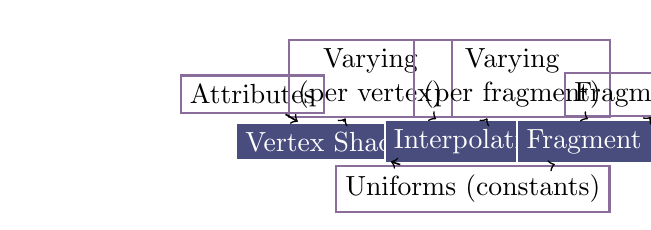
\begin{tikzpicture}[
	node distance = 1cm, on grid,
	mvertex/.style = {draw, rectangle, align=center, draw=H2, color=white, fill=H3, thick},
	vertex/.style = {draw, rectangle, align=center, draw=H1, thick},
  every edge/.style={draw, ->, auto, semithick}
]
  % Define vertices
  \node[vertex] at (0, 0) (attr) {Attributes};
  \node[mvertex] at (1, -0.6) (vs) {Vertex Shader};
  \node[vertex] at (1.5, 0.2) (vvar) {Varying \\ (per vertex)};
  \node[mvertex] at (2.8, -0.6) (inter) {Interpolation};
  \node[vertex] at (3.3, 0.2) (fvar) {Varying \\ (per fragment)};
  \node[mvertex] at (4.8, -0.6) (fs) {Fragment Shader};
  \node[vertex] at (5.3, 0) (fc) {Fragment Color};
  \node[vertex] at (2.8, -1.2) (unif) {Uniforms (constants)};

  \draw (unif) edge (vs);
  \draw (unif) edge (fs);
  \draw (attr) edge (vs);
  \draw (vs) edge (vvar);
  \draw (vvar) edge (inter);
  \draw (inter) edge (fvar);
  \draw (fvar) edge (fs);
  \draw (fs) edge (fc);
\end{tikzpicture}

\begin{definition}[Fragment]
  Fragment \(\neq\) Pixel! A fragment can store:
  \begin{itemize*}
    \item color
    \item position
    \item depth
    \item depth
    \item texture coordinates
    \item window id
    \item \(\sdots\)
  \end{itemize*}
\end{definition}

\begin{definition}[Graphics API]
  Access to hardware with universal interface.
\end{definition}

\section{Light and Colors}

\begin{definition}[Light]
  Electromagnetic radiation (x-rays, micro-, radiowaves). Can be a mixture of many wavelengths.
\end{definition}

\begin{definition}[Color]
  \(P(\lambda)\) = intensity at wavelength \(\lambda\). \(P\) is the \textit{spectral power distribution} (SPD), which we perceive as color, by projecting this spectrum onto a lower-dimensional subspace.
\end{definition}

\subsection{Human Color Perception}

\begin{definition}[Cones]
    {\color{blue} S-short},
    {\color{green} M-medium},
    {\color{red} L-long} wavelength cones.
    \[P(\lambda) \to \left(\int\limits_{380nm}^{780nm}P(\lambda){\color{blue}S}(\lambda), \int\limits_{380nm}^{780nm}P(\lambda){\color{green}M}(\lambda), \int\limits_{380nm}^{780nm}P(\lambda){\color{red}L}(\lambda)\right)\]
    Thus project light into visible 3D-subspace.
\end{definition}

\begin{definition}[Metamers]
  Light with different spectrum map to same color.
\end{definition}

\subsection{CIE Primary System}

\begin{definition}[Primaries]
  Three \textit{single} frequency lights.
  \(\color{red} r(\lambda) = \delta(\lambda - 700)\), \(\color{green}g(\lambda) = \delta(\lambda - 546.1)\) and \(\color{blue}b(\lambda) = \delta(\lambda - 435.8)\).
\end{definition}

Experiment tried to find color matching functions for the mixture of these primaries to generate any reference light:
\[\delta(\lambda - v) \hat{=} \overline{r}(v)r(\lambda) + \overline{g}(v)g(\lambda) + \overline{b}(v) b(\lambda)\]

\(\overline{r}\), \(\overline{g}\), \(\overline{b}\) denote the color target matching functions. Thus we get:
\begin{align*}
  P(\lambda) &= \int P(v)\delta(\lambda - v)dv \\
  &= \left({\color{red}\int P(v)\overline{r}(v)dv}\right)\cdot r(\lambda) + {\color{green}G} \cdot g(\lambda) + {\color{blue}B} \cdot b(\lambda)
\end{align*}

We get negative values for \(R\)! Thus add red to reference light.

\subsection{CIE XYZ Color Space}
Basis transformation of RGB space to represent \textit{all perceptible} colors with new \textit{imaginary} primaries:
\(X = \int_{380}^{780} P(\lambda)\overline{x}(\lambda) d\lambda\), \(Y = \int_{380}^{780} P(\lambda)\overline{y}(\lambda) d\lambda\) and \(Z = \int_{380}^{780} P(\lambda)\overline{z}(\lambda) d\lambda\).

\begin{theorem}
  Value ranges: \(X \in [0, 1.2], Y \in [0, 1], Z \in [0, 1.6]\)
\end{theorem}

\begin{definition}[xyY Color Space]
  Normalization of XYZ space, where \((x, y)\) characterize chromaticity and \(Y\) characterizes brightness.
\end{definition}

\begin{theorem}
  Value ranges: \(x \in [0, 0.75], y \in [0, 0.86], Y\) see XYZ.
\end{theorem}

\pagebreak
\textbf{CIE Chromaticity Diagram}
\vspace{-10pt}
\begin{multicols}{2}
  \includegraphics*[width=\linewidth]{assets/chromaticity.png}
  
  \begin{definition}[Color Gamut]
     Linear combination of 3 colors in \(\triangle\).
  \end{definition}

  \begin{definition}[Purple Line]
    Non-spectral colors between 380 and 770.
  \end{definition}

  \begin{definition}[Dominant Wavelength]
    From color through whitepoint, boundary intersection.
  \end{definition}

  \begin{definition}[Saturation]
    Distance from color to white point.
  \end{definition}

  \begin{definition}[Isoline]
    Line with constant distance to border (w/o PL).
  \end{definition}
\end{multicols}

\vspace{-10pt}
\subsection{Other Color Spaces}

\begin{definition}[RGB]
  Based on three primaries. Used in monitors. Does not cover the whole XYZ space.
\end{definition}

\begin{theorem}
  Value ranges: \(R, G, B \in [0, 1]\)
\end{theorem}

\begin{definition}[CMY]
  Used in passive color systems (printers) and is the inverse to RGB.
  \textit{CMYK} adds black as color.
\end{definition}

\begin{definition}[YIQ]
  Advantages for natural and skin color. Y = Luminance, I = In-Phase (orange-blue) and Q = quadrature (purple-green) components.
\end{definition}

\begin{definition}[HSV]
  Used for interactive color picking.
  Dimensions no longer primaries:
  \textit{Hue} = base color, \textit{saturation} = purity of color and \textit{value/lightness/brightness}. Take RGB, CMY cubes and project to hexagon.
\end{definition}

\begin{theorem}
  Hue \(\in [0, 360]\), Saturation \& Value \(\in [0, 100]\)
\end{theorem}

\begin{definition}[CIELAB/CIELUV]
  Perceptually "uniform": color difference can be measured as distance in chart.
  \textbf{MaxAdams ellipses} become nearly circular.
\end{definition}

\subsection{Transformations}

\begin{definition}[RGB \(\to\) XYZ]
  \[\begin{bmatrix}
    \overline{x}(\lambda) \\ \overline{y}(\lambda) \\ \overline{z}(\lambda)
  \end{bmatrix} = \begin{bmatrix}
    2.36 & -0.515 & 0.005 \\ -0.89 & 1.426 & 0.014 \\ -0.46 & 0.088 & 1.009
  \end{bmatrix} \begin{bmatrix}
    \overline{r}(\lambda) \\ \overline{g}(\lambda) \\ \overline{b}(\lambda)
  \end{bmatrix}\]
\end{definition}

\begin{definition}[XYZ \(\to\) xyY]
  \[x = \frac{X}{X + Y + Z} \quad y = \frac{Y}{X + Y + Z} \quad Y = Y \quad \color{H3}X = \frac{xY}{y} \quad Z = \frac{(1 - x - y)Y}{y}\]
\end{definition}

\begin{definition}[RGB \(\to\) CMY]
  \(\begin{bmatrix}
    C \ M \ Y
  \end{bmatrix}^\top = \begin{bmatrix}
    1 \ 1 \ 1
  \end{bmatrix}^\top - \begin{bmatrix}
    R \ G \ B
  \end{bmatrix}^\top\)
\end{definition}

\begin{definition}[CMY \(\to\) CMYK]
  \(K = \min(C, M, Y), c \in \{C, M, Y\}: c' = c - K\)
\end{definition}

\begin{definition}[RGB \(\to\) YIQ]
  \[\begin{bmatrix}
    Y \\ I \\ Q
  \end{bmatrix} = \begin{bmatrix}
    0.299 & 0.587 & 0.114 \\ 0.596 & -0.275 & -0.321 \\ 0.212 & -0.523 & 0.311
  \end{bmatrix} \begin{bmatrix}
    R \\ G \\ B
  \end{bmatrix}\]
\end{definition}

\begin{definition}[RGB \(\to\) HSV] \
  % \vspace{-8pt}
  % \lstset{basicstyle=\ttfamily\footnotesize,breaklines=true}
  % \begin{center}
  %   \begin{lstlisting}
  % min = min(R, G, B)
  % max = max(R, G, B)
  % V = max;
  % If (max != 0) S = (max - min) / max
  % Else S = 0;
  % H = Hue (V, S, R, G, B); // proced.
  %   \end{lstlisting}
  % \end{center}
  \[C_{\max} = \max(R, G, B) \quad C_{\min} = (R, G, B) \quad \Delta = C_{\max} - C_{\min}\]

  \resizebox{\linewidth}{!}{
    \(
    H = \begin{cases}
        \frac{\pi}{3} \cdot \left(\frac{G - B}{\Delta} \mod 6 \right) & C_{\max} = R \\
        \frac{\pi}{3} \cdot \left(\frac{B - R}{\Delta}    + 2 \right) & C_{\max} = G \\
        \frac{\pi}{3} \cdot \left(\frac{R - G}{\Delta}    + 4 \right) & C_{\max} = R
    \end{cases}
    \
    \begin{array}{c}
    S = \begin{cases}
        0 & C_{\max} = 0 \\
        \frac{\Delta}{C_{\max}} & C_{\max} \neq 0
    \end{cases} \\
        V = C_{\max}
    \end{array}
    \)
  }

\end{definition}

\begin{definition}[HSV \(\to\) RGB]
  \[C = V \cdot S \qquad X = C \cdot \left(1 - \left|\frac{H}{\sfrac{\pi}{3}} mod 2 - 1\right|\right) \qquad m = V - C\]

  \resizebox{\linewidth}{!}{
    \(
    (R', G', B') = \begin{cases}(C, X, 0) & , 0^{\circ} \leq H< \sfrac{\pi}{3} \\ (X, C, 0) & , \sfrac{\pi}{3} \leq H< \sfrac{2\pi}{3} \\ (0, C, X) & , \sfrac{2\pi}{3} \leq H< \pi \\ (0, X, C) & , \pi \leq H< \sfrac{4\pi}{3} \\ (X, 0, C) & , \sfrac{4\pi}{3} \leq H<\sfrac{5\pi}{3} \\ (C, 0, X) & , \sfrac{5\pi}{3} \leq H<2 \pi\end{cases}
    \qquad
    \begin{array}{c}
        R = R' + m \\
        G = G' + m \\
        B = B' + m
    \end{array}
    \)
  }
\end{definition}

 \pagebreak
\section{Transformations}

Transformations map geometry (change position, etc.)

\begin{definition}[Affine Transform]
  \(Ax + b\)
\end{definition}

\begin{definition}[Linear]
  \(Ax\)
\end{definition}

\begin{definition}[Rigid]
  \(Ax + b\) with \(A^{-1} = A^\top\), \(\det(A) = 1\). Translate, Rotate.
\end{definition}

\begin{definition}[Homogeneous Coordinates]
  Used to represent translation using matrix multiplication. \(p = \begin{bmatrix}
    x & y & 1
  \end{bmatrix}^\top\)
\end{definition}

\begin{theorem}
  A point has \(\infty\) homogeneous coords \(p = (wx, wy, w)^\top\).
  Thus normalize by dividing through \(w\).
\end{theorem}

\subsection{2D Transformations}

\makecell{
  \textbf{Translation} \\
  \(\begin{bmatrix}
    1 & 0 & t_x \\ 0 & 1 & t_y \\ 0 & 0 & 1
  \end{bmatrix}\)
}
\makecell{
  \textbf{Scale} \\
  \(\begin{bmatrix}
    s_x & 0 & 0 \\ 0 & s_y & 0 \\ 0 & 0 & 1
  \end{bmatrix}\)
}
\makecell{
  \textbf{Rotation} \\
  \(\begin{bmatrix}
    \cos \theta & - \sin \theta & 0 \\ \sin \theta & \cos \theta & 0 \\ 0 & 0 & 1
  \end{bmatrix}\)
}
\makecell{
  \textbf{Sheer X} \\
  \(\begin{bmatrix}
    1 & a & 0 \\ 0 & 1 & 0 \\ 0 & 0 & 1
  \end{bmatrix}\)
}
\makecell {
  \textbf{Rotation around point} \\
  \(\begin{bmatrix}
    \cos \theta & -\sin \theta & -a \cos \theta + b \sin \theta + a \\
    \sin \theta & \cos \theta & -a \sin \theta - b \cos \theta + b \\
    0 & 0 & 1
  \end{bmatrix}\)
}
\makecell{
  \textbf{Sheer Y} \\
  \(\begin{bmatrix}
    1 & 0 & 0 \\ b & 1 & 0 \\ 0 & 0 & 1
  \end{bmatrix}\)
}
\makecell{
  \textbf{Rotation \(\to\) Translation} \\
  \(\begin{bmatrix}
    r_{11} & r_{12} & t_x \\ r_{21} & r_{22} & t_y \\ 0 & 0 & 1
  \end{bmatrix}\)
}
\makecell{
  \textbf{Commutativity 2D} \\
  Translate / Translate \\
  Rotate / Rotate \\
  Scale / Scale \\
  Scale / Rotate \\
}

\subsection{3D-Transformations}
\makecell{
  \textbf{Rotate X} \\
  \(\begin{bmatrix}
    1 & 0 & 0 & 0 \\
    0 & \cos \theta & - \sin \theta & 0 \\
    0 & \sin \theta & \cos \theta & 0 \\
    0 & 0 & 0 & 1
  \end{bmatrix}\)
}
\makecell{
  \textbf{Rotate Y} \\
  \(\begin{bmatrix}
    \cos \theta & 0 & \sin \theta & 0 \\
    0 & 1 & 0 & 0 \\
    - \sin \theta & -0 & \cos \theta & 0 \\
    0 & 0 & 0 & 1
  \end{bmatrix}\)
}
\makecell{
  \textbf{Rotate Z} \\
  \(\begin{bmatrix}
    \cos \theta & - \sin \theta & 0 & 0 \\
    \sin \theta & \cos \theta & 0 & 0 \\
    0 & 0 & 1 & 0 \\
    0 & 0 & 0 & 1
  \end{bmatrix}\)
}
\makecell{
  \textbf{Shear XY} \\
  \(\begin{bmatrix}
    1 & 0 & sh_x & 0 \\
    0 & 1 & sh_y & 0 \\
    0 & 0 & 1 & 0 \\
    0 & 0 & 0 & 1
  \end{bmatrix}\)
}
\makecell{
  \textbf{Shear XZ} \\
  \(\begin{bmatrix}
    1 & sh_x & 0 & 0 \\
    0 & 1 & 0 & 0 \\
    0 & sh_z & 1 & 0 \\
    0 & 0 & 0 & 1
  \end{bmatrix}\)
}
\makecell{
  \textbf{Shear YZ} \\
  \(\begin{bmatrix}
    1 & 0 & 0 & 0 \\
    sh_y & 1 & 0 & 0 \\
    sh_z & 0 & 1 & 0 \\
    0 & 0 & 0 & 1
  \end{bmatrix}\)
}

\textbf{Change of coordinate systems}
\vspace{-10pt}
\begin{multicols}{2}
  \(\begin{bmatrix}
    r_1 & r_2 & r_3 & t \\
    0 & 0 & 0 & 1
  \end{bmatrix} \begin{bmatrix}
    p_x \\ p_y \\ p_z \\ 1
  \end{bmatrix} = p'\)

  \(r_\alpha\) is old \(\alpha\)-axis in new system.
  \(t\) is translation in new system.
  \(p'\) is the new point.
  Basically rotation then translation.
\end{multicols}

\vspace{-10pt}
\begin{definition}[Transforming Normals]
  When \(p' = Mp\), then \(n' = (M^{-1})^\top n\).
\end{definition}

\subsection{Perspective and Projection}
\(d\) is the distance from the camera point:

\makecell{
  \textbf{Perspective Projection} \\
  \(\begin{bmatrix}
    I_{2} & 0 & 0 \\
    0 & 1 & 0 \\
    0 & 1/d & 0
  \end{bmatrix}\)
}
\makecell{
  \textbf{Parallel Projection} \\
  \(\begin{bmatrix}
    I_{2} & 0 & 0 \\
    0 & 0 & 0 \\
    0 & 0 & 1
  \end{bmatrix}\)
}

\(\implies\) Make homogeneous afterwards!

\begin{theorem}
  These transformations are not considered affine!
\end{theorem}

\begin{definition}[Clipping Planes]
  In front of front-clipping-plane and after back-clipping-plane objects are not rendered anymore.
\end{definition}

\pagebreak
\subsection{OpenGL Transformations}

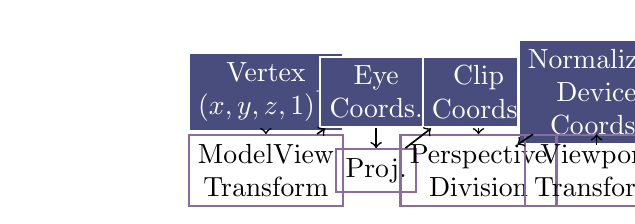
\begin{tikzpicture}[
	node distance = 1cm, on grid,
	mvertex/.style = {draw, rectangle, align=center, draw=H2, color=white, fill=H3, thick},
	vertex/.style = {draw, rectangle, align=center, draw=H1, thick},
  every edge/.style={draw, ->, auto, semithick}
]
  % Define vertices
  \node[mvertex] at (0, 0) (vertex) {Vertex \\ \((x, y, z, 1)^\top\)};
  \node[mvertex] at (1.4, 0) (ec) {Eye \\ Coords.};
  \node[mvertex] at (2.7, 0) (cc) {Clip \\ Coords.};
  \node[mvertex] at (4.2, 0) (ndc) {Normalized \\ Device \\ Coords.};
  \node[mvertex] at (5.6, 0) (wsc) {Window \\ (Screen) \\ Coords.};
  \node[vertex] at (0, -1) (mvt) {ModelView \\ Transform};
  \node[vertex] at (1.4, -1) (proj) {Proj.};
  \node[vertex] at (2.7, -1) (pd) {Perspective \\ Division};
  \node[vertex] at (4.2, -1) (vt) {Viewport \\ Transform};

  % Edges
  \draw (vertex) edge (mvt);
  \draw (mvt) edge (ec);
  \draw (ec) edge (proj);
  \draw (proj) edge (cc);
  \draw (cc) edge (pd);
  \draw (pd) edge (ndc);
  \draw (ndc) edge (vt);
  \draw (vt) edge (wsc);
\end{tikzpicture}

\begin{definition}[Model View Transform]
  First model to world coordinates:
  \begin{center}
    \(\begin{bmatrix}
      r_1 & r_2 & r_3 & t \\ 0 & 0 & 0 & 1
    \end{bmatrix} \begin{bmatrix}
      \rotatebox{90}{model } \\ 1
    \end{bmatrix}  = \begin{bmatrix}
      \rotatebox{90}{world } \\ 1
    \end{bmatrix}\)
  \end{center}
  Then world to camera:

  \begin{center}
    \(\begin{bmatrix}
      \text{left} & \text{up} & \text{-dir} & \text{eye} \\ 0 & 0 & 0 & 1
    \end{bmatrix} \begin{bmatrix}
      \rotatebox{90}{cam } \\ 1
    \end{bmatrix} = \begin{bmatrix}
      \rotatebox{90}{world } \\ 1
    \end{bmatrix}\)
  \end{center}
\end{definition}

\begin{definition}[Projection]
  \ \\
  Either parallel:
  \(\begin{bmatrix}
    \frac{2}{r -l} & 0 & 0 & - \frac{r + l}{r - l} \\
    0 & \frac{2}{t - b} & 0 & - \frac{t + b}{t - b} \\
    0 & 0 & - \frac{2}{n - f} & - \frac{f + n}{f - n} \\
    0 & 0 & 0 & 1
  \end{bmatrix} \begin{bmatrix}
    c \\ 1
  \end{bmatrix} = \begin{bmatrix}
    c' \\ 1
  \end{bmatrix}\)

  Or perspective:
  \
  \(\begin{bmatrix}
    \frac{2n}{r - l} & 0 & \frac{r + l}{r - l} & 0 \\
    0 & \frac{2n}{t - b} & \frac{t + b}{t - b} & 0 \\
    0 & 0 & - \frac{f + n}{f - n} & - \frac{2 f n}{f - n} \\
    0 & 0 & -1 & 0
  \end{bmatrix} \begin{bmatrix}
    c \\ 1
  \end{bmatrix} = \begin{bmatrix}
    c' \\ -c_z
  \end{bmatrix}\)
\end{definition}

\begin{definition}[Perspective Divison]
  \(\frac{1}{- c_z}c' = \begin{bmatrix}
      d_x & d_y & d_z
  \end{bmatrix}^\top\)
  which are the normalized device coordinates. \(d_x, d_y\) position and \(d_z\) depth.
\end{definition}

\begin{definition}[Viewport Transform]
  \(\text{screen cord.} = \begin{bmatrix}
    \frac{w}{2}d_x + (o_x  + \frac{w}{2}) \\
    \frac{h}{2}d_y + (o_y + \frac{h}{2}) \\
    \frac{f - n}{2}d_z + \frac{f + n}{2}
  \end{bmatrix}\)
\end{definition}

\section{Lighting}

\begin{definition}[Lighting]
  Modeling physical interaction between materials and light sources.
\end{definition}

\begin{definition}[Radiometry]
  Studies measurement of radiation (w/ lighting).
\end{definition}

\begin{definition}[Angle]
  \(\theta = \frac{\text{arc-length}}{r}\), for circle \(2 \pi\) radians.
\end{definition}

\begin{definition}[Solid Angle]
  \(\Omega = \frac{A}{r^2}\).
  For sphere: \(4\pi\) steradians.
\end{definition}

\begin{definition}[Angle]
  Point on unit sphere parameterized by \(\omega = (\theta, \phi)\).

  Zenith and Azimuth.
  Thus \(\text{lat} =\frac{90}{\pi}(\pi - \theta)\) and \(\text{long} = \frac{90}{\pi}\phi\).
\end{definition}

\begin{definition}[Differential Solid Angle]
  \(dA = (rd\theta)(r \sin \theta d \phi)\) as well as
  \(d\omega = \frac{dA}{r^2} = \sin \theta d \theta d \phi\).
\end{definition}

\begin{definition}[Light]
  Photons with position \(x\), direction \(\omega\) and wavelength \(\lambda\).
\end{definition}

\begin{definition}[Photon Energy]
  \(\frac{hc}{\lambda} \ [J]\) with \(h\) being Planck's  constant.
\end{definition}

\subsection{Radiometry}
\begin{definition}[Flux/Radiant Flux/Power]
  \(\Phi(A) \ \left[\frac{J}{s} = W\right]\): amount of energy (\#photons) passing through surface or space per unit time.
\end{definition}

\begin{definition}[Irradiance]
  \(E(x) = \frac{d \Phi(A)}{d A(x)} \ \left[\frac{W}{m^2}\right]\):
  flux per \textit{unit area arriving}.
\end{definition}

\begin{algorithm}[Lambert's Cosine Law]
  \(E =\frac{\Phi}{A / \cos \theta} = \frac{\Phi}{A} \cos \theta = E_{\vec{n}} \cos \theta\).
\end{algorithm}

\begin{definition}[Radiosity]
  \(B(x) = \frac{d\Phi(A)}{dA(x)} \ \left[\frac{W}{m^2}\right]\):
  flux per \textit{unit area leaving}.
\end{definition}

\begin{definition}[Intensity]
  \(I(\omega) = \frac{d\Phi}{d\omega} \ \left[\frac{W}{sr}\right]\):
  Flux per solid angle (direction). Thus \(\Phi = \int_{S^2} I(\omega) d\omega = 4 \pi I\) for an isotropic point source.
\end{definition}

\begin{definition}[Radiance]
  \(L(x, \omega) = \frac{d^2 \Phi(A)}{\cos \theta dA(x) d\omega} \ \left[\frac{W}{m^2sr}\right]\):
  Intensity per unit area or flux density per unit solid angle, per perpendicular unit area. Most fundamental in raytracing!
\end{definition}

\subsection{Reflection Models}
\begin{definition}[BRDF]
  Bidirectional reflectance distribution function. Relationship between incident radiance and differential reflected radiance. \(\omega_i\) = incoming angle, \(\omega_r\) reflected angle.
  \[f_r(x, \omega_i, \omega_r) = \frac{dL_r(x, \omega_r)}{dE_i(x, \omega_i)} = \frac{dL_r(x, \omega_r)}{L_i(x, \omega_i) \cos \theta_i d\omega_i}\]
\end{definition}

\begin{definition}[Reflection Equation]
  Describes \textit{local illumination} model to compute the reflected radiance. \(H^2\) is the hemisphere.
  \[L_r(x, \omega_r) = \int_{H^2}f_r(x, \omega_i, \omega_r)L_i(x, \omega_i) \cos \theta_i d \omega_i\]
\end{definition}

\includegraphics*[width=\linewidth]{assets/reflections.png}

\begin{definition}[Diffuse Reflection]
  For diffuse reflection, the BRDF is a constant.
  \(L_r(x) = f_r E_i(x)\).
\end{definition}

\begin{algorithm}[Phong Illuminiation Model]
  \[I_\lambda = \underbrace{I_a k_a}_{\text{Ambient}} + f_{att}I_p[\underbrace{k_d(N \cdot L)}_{\text{Diffuse}} + \underbrace{k_s(R \cdot V)^n}_{\text{Specular}}]\]
  \begin{itemize}
    \item \textit{Material param}: \(k_a, k_d, k_s,\) \(n\) specular size
    \item \textit{Light param}: \(I_a\) global ambient, \(I_p\) light intensity
    \item \textit{Geometry}: \(N\) face normal, \(L\) light pos, \(V\) camera pos
  \end{itemize}
\end{algorithm}

\begin{theorem}
  For multiple lights, sum diffuse/specular for each light.
\end{theorem}

\begin{definition}[Ambient]
  Light inherent in scene \(\approx\) global illuminiation.
\end{definition}

\begin{definition}[Diffuse]
  Reflection on matt, dull surfaces. Follows Lambertian's law.
  \(I = I_pk_d\cos \theta = I_p k_d(N \cdot L)\).
\end{definition}

\begin{definition}[Specular]
  Reflection on shiny surfaces. Depends on angle between the reflection and viewing ray. \(R=2N(N \cdot L) - L\).
\end{definition}

\begin{theorem}
  Using halfway vectors would be faster to compute the cosine power: \(\cos^n \beta = (N \cdot H)^n\) with \(H = \frac{L + V}{||L + V||}\).
\end{theorem}

\begin{definition}[Attenuation]
  Quadratic due to spatial radiation. \(f_{att} = (d_L^2)^{-1}\) or often used in OpenGL:
  \(f_{att} = \min((c_1 + c_2d_L + c_3d_L^2)^{-1}, 1)\)
\end{definition}

\section{Shading}

\begin{definition}[Shading]
  Process of determining the color of a pixel.
\end{definition}

\begin{definition}[Flat Shading]
  One color per primitive. Screen space shading.
\end{definition}

\begin{theorem}
  Color is a per vertex attribute normally!
\end{theorem}

\begin{algorithm}[Gouraud Shading]
  Linear interpolation of vertex intensities. Screen space shading.
  \begin{enumerate}
    \item Calculate face normals
    \item Calculate vertex normal by averaging
    \item Interpolate vertex color bilinearly on current scan line.
  \end{enumerate}

  \textit{Problems}:
  \begin{itemize*}
    \item perspective distortion
    \item orientation dependence
    \item shared vertices
    \item quality depends on vertices
  \end{itemize*}
\end{algorithm}


\begin{algorithm}[Phong Shading]
  Barycentric interpolation of normal on the triangle. Thus color of fragment \(x\) is determined by interpolated normals.

  \textit{Problems}:
  \begin{itemize*}
    \item Normal not defined/representative.
  \end{itemize*}
\end{algorithm}

\subsection{Transparency}

Use \textbf{RGBA} channels to calculate the overlapping objects.

\begin{algorithm}[Alpha Blending]
  Linearizes exponential attenuation of light intensity. \(I_\lambda = I_A \alpha_1 \Delta t + I_Be^{-\alpha_1\Delta t} \approx I_A \alpha_1 + I_B(1 - \alpha)\). Where object \(A\) is in front of \(B\) and has a thickness of \(\Delta t\).
\end{algorithm}

\begin{definition}[Back to front rendering]
  Sorted traversal of polygons from back to front.
  \textit{Problems}: overlapping objects.
\end{definition}

\begin{definition}[Depth peeling]
  Multiple passes which render the next closest fragment.
\end{definition}

\section{Geometry \& Textures}
\begin{definition}[Sources of Geometry]
  \begin{itemize*}
    \item 3D Scanning
    \item Point clouds
    \item 3D modeling
    \item procedural modeling
  \end{itemize*}
\end{definition}

\subsection{Geometric Representations}

\begin{definition}[Parametric Surfaces]
  i.e. \(f(x, y , z) = 0\).
  \begin{itemize*}
    \item implicit
    \item simple storage
    \item fast in/out test
    \item only works for easy surfaces
  \end{itemize*}
\end{definition}

\begin{definition}[Subdivision surfaces]
  \begin{itemize*}
    \item implicit
    \item surface piecewise linear
    \item increase sub.div. for more precision
  \end{itemize*}
\end{definition}

\begin{definition}[Point Set]
  \begin{itemize*}
    \item explicit
    \item collection of points
    \item \color{red} difficult to draw in undersampled regions
    \item \color{red} hard to do processing / simulation
  \end{itemize*}
\end{definition}

\begin{definition}[Polygonal Meshes]
  \begin{itemize*}
    \item explicit
    \item boundary of objects
    \item geometry + connectivity
    \item attributes (color, normals, \(\sdots\))
    \item fast on GPU
    \item should support rendering, geometry queries, modifications
  \end{itemize*}
\end{definition}

\begin{definition}[Implicit Surface]
  Created by some method: level-set and signed distance function.
\end{definition}

\subsection{Mesh Datastructures}

\begin{definition}[Polygon]
  \(\langle V, E\rangle\), planar and non self-intersecting.
\end{definition}

\begin{definition}[Polygonal Mesh]
  \(M = \langle V, E, F\rangle\).
  \textit{Properties}:
  \begin{itemize*}
    \item every edge belongs to at least one polygon
    \item intersection of two polygons in \(M\) is either empty, a vertex, or an edge.
  \end{itemize*}
\end{definition}

\begin{definition}[Valence]
  Number of edges incident to a vertex
\end{definition}

\begin{definition}[Boundary]
  The set of all edges that belong to only 1 polygon.
\end{definition}

\begin{definition}[Manifold]
  Surface locally homeomorphic to a disk. Closed manifolds divide space into two.
\end{definition}

\begin{definition}[Triangle List]
  List of triangles.
  \begin{itemize*}
    \item simple
    \item no connectivity
    \item redundant
    \item STL file format
    \item easy queries
  \end{itemize*}
\end{definition}

\begin{definition}[Indexed Face Set]
  Two arrays, one describes the triangles with vertex indices and the index array contains the coordinates per vertex index.
  \begin{itemize*}
    \item avoids redundancy
    \item stores connectivity (costly geometric queries and mesh modifications)
    \item OBJ, OFF, WRL
  \end{itemize*}
\end{definition}

\subsection{Maps}

\begin{definition}[Texture Mapping]
  Increase detail without more geometry.

  \textit{Desirable}:
  \begin{itemize*}
    \item low distortion
    \item bijective
    \item efficient to compute
  \end{itemize*}

  \textit{Issues}:
  \begin{itemize*}
    \item texture atlases
    \item finding cuts
    \item anti-aliasing
    \item details
  \end{itemize*}
\end{definition}

\begin{theorem}
  Sphere Param:
  \((u, v)^\top \to (\sin u \sin v, \cos v, \cos u \sin v)^\top\)
\end{theorem}

\begin{theorem}
  Mapping textures could cause aliasing \(\to\)
  Use LPF, but isotropic Gauss in screen space is anisotropic in texture space.
  Use an anisotropic spatially-varying texture filter.
\end{theorem}

\begin{definition}[Anisotropic Gauss]
  \[f(x, y) = \frac{1}{2 \pi \sigma_x \sigma_y}\exp\left(- \left(\frac{x^2}{2 \sigma^2_x} + \frac{y^2}{2 \sigma_y^2}\right)\right)\]
\end{definition}

\begin{theorem}
  Textures can be procedurally generated via \textbf{Perlin noise} or \textbf{Gabor noise} (more control over spectral properties)
\end{theorem}

\begin{definition}[Solid Textures]
  Textures for each 3D coordinate.
\end{definition}

\begin{definition}[Light Map]
  Brightness map, similar to texture mapping.
\end{definition}

\begin{definition}[Environment Map]
  For reflective objects. Intersect ray with surrounding sphere/cube instead of scene. Really fast.
\end{definition}

\begin{definition}[Bump Mapping]
  Positional peturbation in direction of normal!
  small-scale geometry per fragment.
  Does not affect silhouette shadow.
  No self-occlusions and self-shadowing.
\end{definition}

\begin{definition}[Displacement Map]
  Per vertex, changes actual geometry.
\end{definition}

\begin{definition}[Normal Map]
  Each pixel has its own normal.
  For each pixel: \(n' = (2r - 1, 2g - 1, 2b - 1)^\top\).
\end{definition}

\begin{theorem}
  Normals are stored in texture space \((u, v, n)\) and thus need to be transformed into the object space \((N, T, B)\).
  Each point \(p = (x, y, z)^\top\) has linear relation \(A\) to its texture coordinate \(\vec{u} = (u, v)^\top\).
  For each triangle compute Tangent and Bitangent.
  \(T\) and \(B\) correspond to \((1, 0)\) and \((0, 1)\) in texture space:
  \[p = A \vec{u} \to \begin{bmatrix}
    \vec{T} & \vec{B}
  \end{bmatrix} = A I_{2 x 2} = A\]
  For triangle \(p_1, p_2, p_3\) got two conditions:
  \[p_2 = A \vec{u}_2 \ \land \ p_3 = A \vec{u}_3 \implies \begin{bmatrix}
    p_2 & p_3
  \end{bmatrix} = A \begin{bmatrix}
    \vec{u}_2 & \vec{u}_3
  \end{bmatrix}\]
  Solve for \(A\) and you got \(\begin{bmatrix}
    \vec{T} & \vec{B}
  \end{bmatrix}\).
\end{theorem}

\begin{definition}[Mip Map]
  Store texture with image pyramid. Choose res based on projected size of triangle. LERP in-between depths.
\end{definition}

\section{Scan Conversion (Rasterization)}

Approximation of a primitive by a finit number of pixels.

\begin{algorithm}[Bresenham Line]
  Fast decision which pixel has to be drawn next.
  \textit{Criterion}: Position of midpoint \(m\) to intersection \(q\).
  Consider the line equation: \(f(x, y) = ax + by + c = 0\): 

  \begin{enumerate}
    \item \(d = f(m) = f(x_p + 1, y_p + 1/2) > 0 \implies\) NE, else E
    \item NE \(\implies d_{new} = d_{old} + \Delta y - \Delta x\), else \(d_{new} = d_{old}+ \Delta y\).
  \end{enumerate}
\end{algorithm}

\begin{theorem}
  For polygons an inside test for each px is too inefficient.
\end{theorem}

\begin{definition}[Polygon Span]
  Group of (neighboring) px's within scan line.
\end{definition}

\begin{algorithm}[SC of Polygons]
  \begin{enumerate}
    \item Calc all intersections on scan line
    \item Sort intersection points by ascending \(x\)-coordinate
    \item Fill all spans in between two consecutive intersections points if the parity is odd.
  \end{enumerate}
\end{algorithm}

\section{Splines}

\begin{definition}[Local Coordinate System]
  \(u \in \R: x(u) = (x(u), y(u), z(u))^\top\)
  Thus map the 1D param space into 3D or 2D.
\end{definition}

\subsection{Bézier Curves}

\begin{center}
  \(x(t) = b_0B_0^n(t) + \ldots + b_n B_n^n(t)\) where \(b_i \in \R^3\)
\end{center}

\begin{itemize}
  \item \textbf{Affine invariance}: Affine transform of all points is accomplished by the affine transform of its control points.
  \item \textbf{Convex Hull Property}: The curve lies in the convex hull.
  \item Control polygon gives rough sketch of curve.
  \item \textbf{Endpoint interpolation}, since \(B_0^n(0) = B_n^n(1) = 1\)
  \item \textbf{Variation diminishing property}: Maximum number of intersections of a line with the curve is less or equal to the number of intersection with its control polygon.
  \color{red}
  \item \textbf{Global Support}: Control points influence whole curve.
  \item Insertion of new control point comes along with degree evaluation.
\end{itemize}

\begin{definition}[Control Point]
  Points defining the hull of the spline: \(b_i\).
\end{definition}

\begin{definition}[Bernsteinpolynomial]
  \(B_i^n(t) = \binom{n}{i} t^i(1 - t)^{n-1}\), \(i \notin [1, n]: 0\)

  \textit{Properties}:
  \begin{itemize*}
    \item Partition of unity (meaning at every point the sum of polynomials is 1)
    \item positive definite
    \item recursion
    \item symmetry
  \end{itemize*}
\end{definition}

\begin{definition}[Polynomial Degree]
  Highest exponent of the polynomial = number of control points.
\end{definition}

\begin{definition}[Polynomial Order]
  order = degree + 1
\end{definition}

\begin{theorem}
  Cubic Bézier curve has 4 control points!
\end{theorem}

\begin{algorithm}[DeCasteljau Algorithm]
  \lstset{
    basicstyle=\small\ttfamily,
    language=Pascal,
    captionpos=b
  }
  Interpolation in \(\O(n^2)\) \vspace{-5pt}
  \begin{lstlisting}[mathescape=true]
fun DeCasteljau(t, {b_0, b_1, ..., b_n}):
  for i from n to 1 do
    for j from 0 to i-1 do
      $b_j$ = (1 - t) * $b_j$ + t * $b_{j+1}$
  return $b_0$ // Final interpolated point
\end{lstlisting}
Basically interpolate, till you no longer can interpolate. If you write \(b_0\) out and factor out the original control points, you get the sum of Bernsteinpolynomials again.
\end{algorithm}

\begin{theorem}
  Derivative is another Bézier of order \(n-1\).
\end{theorem}

\begin{theorem}
  Combining Bézier curves makes the whole curve \(C^0\).
\end{theorem}

\begin{definition}[Piecewise Bézier Curves]
  Two composed Bézier curves (e.g. segments \(b_0, \ldots b_n\) in \([u_0, u_1]\) and \(b_n, \ldots b_{2n}\) in \([u_1, u_2]\)) need the following constraint to enforce \(C^r\)-continuity:
  \(b_{n+i} = b_{n-i}^i(t)\) for \(i = 0, \ldots, r\) where \(t = (u - u_0) / (u_1 - u_0)\) stands for the local coordinate of \(u_2\) relative to \(u_0, u_1\).
\end{definition}

\begin{definition}[Joining Cubic Béziers]
  Curve \(A \cup B\) is \(C^n\) continuous if segment \(A^{(i)}(t_{end}) = B^{(i)}(t_{start})\) for \(i = 0, \ldots n\).
\end{definition}

\begin{theorem}
  Thus for \(C^1\), we need \(b_{n-1}\) to be mirrored on \(b_n\) by \(b_{n+1}\).
\end{theorem}

\begin{definition}[Matrix Form]
  We can rewrite the curve equation with vectors:
  \(x(t) = \sum_i^n b_i B_i^n(t) = (b_0, \sdots, b_n)(B_0^n(t), \sdots, B_n^n(t))^\top\).
  Then we use a basis transformation to get a monomial representation:
  \[\begin{bmatrix}
    B_0^n(t) \\ \vdots \\ B_n^n(t)
  \end{bmatrix} = \begin{bmatrix}
    m_{00} & \ldots & m_{0n} \\ \vdots & & \vdots \\ m_{m0} & \ldots & m_{mn}
  \end{bmatrix} \begin{bmatrix}
    t^0 \\ \vdots \\ t^n
  \end{bmatrix}\]
\end{definition}

\begin{theorem}
  For Bernstein polynomials we get  \(m_{ij} = (-1)^{j-i}\binom{n}{j} \binom{j}{i}\).
\end{theorem}

\begin{definition}[Spline Interpolation]
  Interpolate \(\{p_0, \ldots, p_n\}\) with \(x(t_i) = p_i\).
  
  \begin{center}
    \(\begin{bmatrix}
      1 & t_0 & \ldots & t_0^n \\ \vdots & \vdots & & \vdots \\ 1 & t_n & \ldots & t_n^n
    \end{bmatrix} \begin{bmatrix}
      a_0 \\ \vdots \\ a_n
    \end{bmatrix} = \begin{bmatrix}
      p_0 \\ \vdots \\p_n
    \end{bmatrix}\)
  \end{center}

  Where \(a_i\) are the polynomial coefficients.
\end{definition}

\subsection{B-Spline Curves}

\begin{center}
  \(s(u) = \sum_{i=0}^n d_i N_i^n(u)\) where \(d_i \in \R^3\)
\end{center}

Coefficients \(d_i\) are \textit{de Boor} points. Bases are piecewise, recursively defined polynomials over a sequence of knots defined in the knot vector \(T = (u_0, \ldots, u_{k+n+1})\).

\begin{itemize}
  \item Different degrees
  \item Piecewise polynomial
  \item Local support (de Boor points only have local influence)
  \item uniform/non-uniform (distance from \(u_i\) to \(u_{i+1}\))
\end{itemize}

\begin{definition}[B-Spline Functions]
  \[N_i^n(u) = (u - u_i)\frac{N_i^{n-1}(u)}{u_{i+n} - u_i} + (u_{i+n+1} - u)\frac{N_{i+1}^{n-1}(u)}{u_{i+n+1} - u_{i+1}}\]
  where \(N_i^0(u) = \begin{cases}
    1 & u \in [u_i, u_{i+1}] \\ 0 & \text{otw.}
  \end{cases}\)

  \textit{Properties}:
  \begin{itemize*}
    \item Partition of unity
    \item Positivity (\(N_i^n(u) \geq 0\))
    \item Compact (\(N_i^n(u) = 0, u \notin [u_i, u_{i+1}]\))
    \item Continuity (\(N_i^n\) is \(C^{n-1}\)).
  \end{itemize*}
\end{definition}

\begin{definition}[B-Spline filters]
  Cardinal B-Splines over uniform knot sequences can be computed using the convolution:
  \[N_i^n = N^{n-1} \ast N^0 \quad N^0: \text{box} - \text{function}\]
\end{definition}

\begin{theorem}
  Curve is globally \(C^{n-1}\) except multiple knots of order \(p\) with \(u_j = \ldots u_{j+p-1}\) lead to \(C^{n-p}\).
\end{theorem}

\begin{algorithm}[deBoor Algorithm]
  Successive linear interpolation:
  \[d_i^k = (1 - a_i^k)d_{i-1}^{k-1} + a_i^k d_i^{k-1} \quad a_i^k = \frac{t - u_i}{u_{i+n+1-k} - u_i}\]
  where \(d_i^0 = d_i\) and \(d_n^n = s(t)\).
\end{algorithm}

\begin{theorem}
  With first and last knot multiplicity of \(n+1\) we have that the deBoor Algorithm = DeCasteljau Algorithm.
\end{theorem}

\begin{definition}[Spline Interpolation]
  System is under-determined. Need \(k+n\) control points to interpolate \(k+1\) points. \(k-1\) define the interior intervals and \(n+1\) the boundaries.
\end{definition}

\subsection{Tensor Product Surfaces}
From curve to a surface involves taking a tensor product.
\[x(u, v) = \sum_{i=0}^{n}\sum_{j=0}^{m}\alpha_{i, j} F_i(u)G_j(v)\]

\begin{definition}[Bézier Patches]
  \(F_i = B_i^m\) and \(G_j = B_i^n\).

  \textit{Properties}:
  \begin{itemize*}
    \item Affine invariance
    \item convex hull property
    \item variation diminishing property
    \item boundary curves (patch boundaries are Bézier curves)
  \end{itemize*}
\end{definition}

\begin{algorithm}[2D DeCasteljau]
  There exists the 2D DeCasteljau algorithm.
\end{algorithm}

\begin{definition}[Warping as a 2D Parametric Function]
  Given a matrix of vector valued landmark points:
  \[m(u_i, v_j) = \begin{bmatrix}
    B_0(u_i) & \ldots & B_n(u_i)
  \end{bmatrix} \begin{bmatrix}
    b_{00} & \ldots & b_{0m} \\ \vdots && \vdots \\ b_{n0} & \ldots & b_{nm}
  \end{bmatrix} \begin{bmatrix}
    B_0(v_j) \\ \vdots \\ B_m(v_j)
  \end{bmatrix}\]
  Solve this interpolation problem.
\end{definition}

\begin{definition}[Matrix Form]
  Same as in 1D. Rewrite in monomial basis:
  \[b^{m, n}(u, v) = (u^0, \ldots, u^m)M^\top[b_{ij}]_{i\in[m], j\in[n]}N (v^0, \ldots, v^n)^\top\]
  With \(m_{ij} = (-1)^{j - i} \binom{m}{j}\binom{j}{i}\) and \(n_{ij} = (-1)^{j - i} \binom{n}{j}\binom{j}{i}\)
\end{definition}

\begin{definition}[B-Spline Patches]
  \(F_i = N_i^n\) and \(G_j = M_j^m\).
\end{definition}

\begin{algorithm}[2D DeBoor Algorithm]
  It exists :)
\end{algorithm}

\begin{definition}[Rational B-Spline Patches (Nurbs)]
  Most advanced modelling and animation systems are based on NURBS. They are \textbf{not} tensor product surfaces, since bases are non-separable.
  \[s(u,v) = \frac{\sum_i \sum_j w_{i, j} d_{i, j}N_i^m(u)N_j^n(v)}{\sum_i \sum_j w_{i, j}N_i^m(u)N_j^n(v)}\]
\end{definition}

\section{Subdivision Surfaces}
Generalization of spline curves/surfaces. Used for successive refinement (subdivision) and converges to smooth limit surface. \textit{Control Polygon \(\to\) smooth curve}.

\subsection{Line Subdivision}

\begin{definition}[Curve Types]
  \begin{itemize}
    \item \textit{Approximating}: \begin{enumerate}
      \item Split each edge in two
      \item Relocate each (original) vertex with some simple rule.
    \end{enumerate}

    \item \textit{Interpolating}: \begin{enumerate}
      \item Keep old vertices
      \item Generate new vertices by fitting cubic curve to old vertices
      \item \(C^1\) continuous limit curve.
    \end{enumerate}

    \item \textit{Corner Cutting}: \begin{enumerate}
      \item Insert two new vertices at \(1/4, 3/4\).
      \item Remove old vertices and connect the new ones
    \end{enumerate}
  \end{itemize}
\end{definition}

\begin{definition}[Catmull-Clark Filter]
  Approximating equivalent with: insert new point in mid-edge, then filter with \((1/8, 6/8, 1/8)\).
\end{definition}

\subsection{Surface Subdivision}
\begin{tabular}{|c|c|c|c|}
  \hline & \multicolumn{2}{c|}{ Primal } & \multirow{2}{*}{ Dual } \\
  \cline{2-3} & Triangles & Rectangles & \\
  \hline Approx. & Loop & Catmull-Clark & \multirow{2}{*}{\begin{tabular}{c} 
  Doo-Sabin \\
  Midedge
  \end{tabular}} \\
  \hline Interp. & Butterfly & Kobbelt & \\
  \hline
\end{tabular}

\begin{definition}[Primal]
  Faces are split into sub-faces.
\end{definition}

\begin{definition}[Dual]
  Vertices are split into multiple vertices.
\end{definition}

\begin{definition}[Approximating]
  Control points are not interpolated.
\end{definition}

\begin{definition}[Interpolating]
  Control points are interpolated.
\end{definition}

\begin{theorem}
  Different subdivision rules for each valence.
\end{theorem}

\begin{algorithm}[Doo-Sabin]
  Generalization of Bi-quadratic B-Splines.

  \textit{Applied to}: Polygonal meshes

  \textit{Creates}: \(G^1\) -- \(C^0\) for center of irregular polygons after 1 step and \(C^1\) everywhere else.
\end{algorithm}

\begin{algorithm}[Catmull-Clark]
  Generalization of Bi-cubic B-Splines.

  \textit{Applied to}: Polygonal meshes

  \textit{Creates}: \(G^2\) -- \(C^1\) for \(\text{deg}(v) \neq 4\) and \(C^2\) everywhere else.
\end{algorithm}

\begin{algorithm}[Loop]
  Generalization of box-splines.

  \textit{Applied to}: Triangle meshes

  \textit{Creates}: \(G^2\) -- \(C^2\) for \(\text{deg}(v) \neq 6\) and \(C^2\) everywhere else.
\end{algorithm}

\begin{algorithm}[Butterfly Subdivision]
  \textit{Applied to}: Triangle meshes

  \textit{Creates}: \(G^1\) -- \(C^0\) for \(\text{deg}(v) = 3\) or \(> 7\) and \(C^1\) elsewhere.
\end{algorithm}

\begin{theorem}
  Catmull-Clark \& Loop are the best schemes.
\end{theorem}

\begin{itemize*}
  \item Flexible modeling
  \item Scalability
  \item Usability
\end{itemize*}

\makecell{
  \textbf{Start} \\
  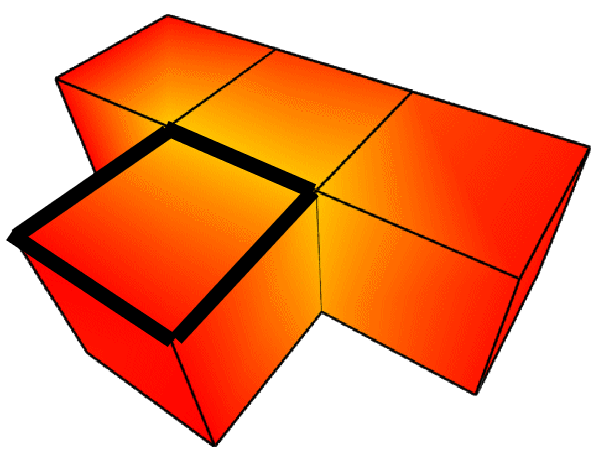
\includegraphics[width=0.3\columnwidth]{assets/start-square.png}
}
\makecell{
  \textbf{Doo-Sabin} \\
  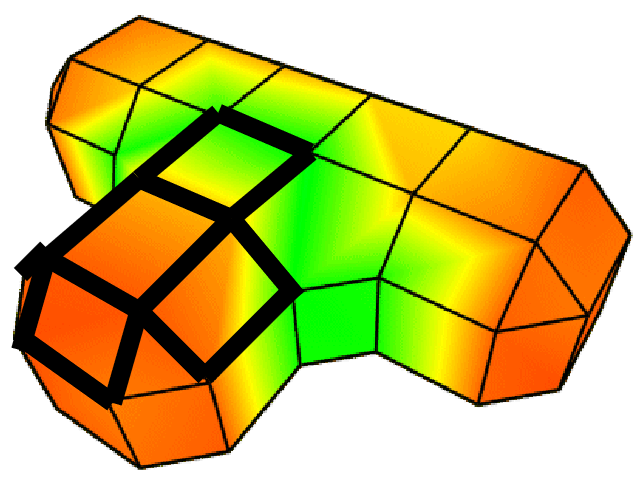
\includegraphics[width=0.3\columnwidth]{assets/doo-sabin.png}
}
\makecell{
  \textbf{Catmull-Clark} \\
  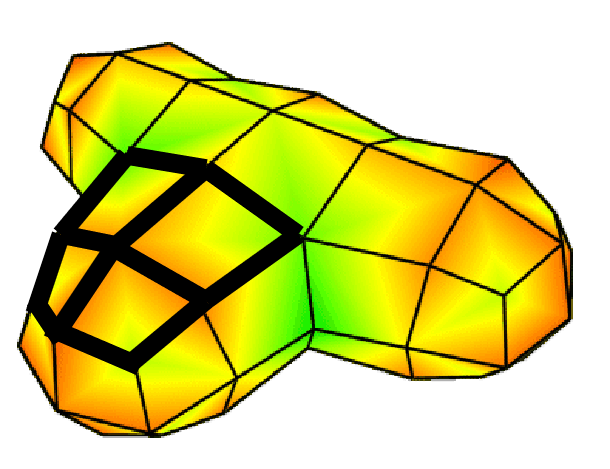
\includegraphics[width=0.3\columnwidth]{assets/catmull-clark.png}
}
\makecell{
  \textbf{Start} \\
  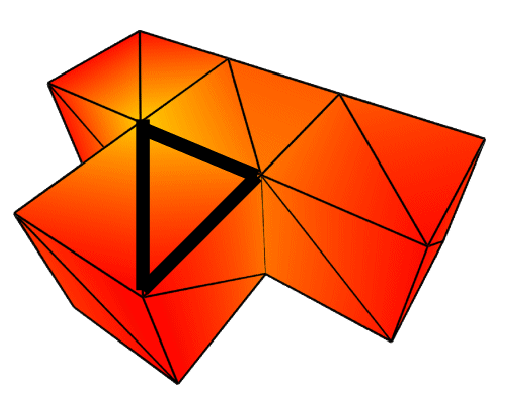
\includegraphics[width=0.3\columnwidth]{assets/start-triangle.png}
}
\makecell{
  \textbf{Loop Subdivision} \\
  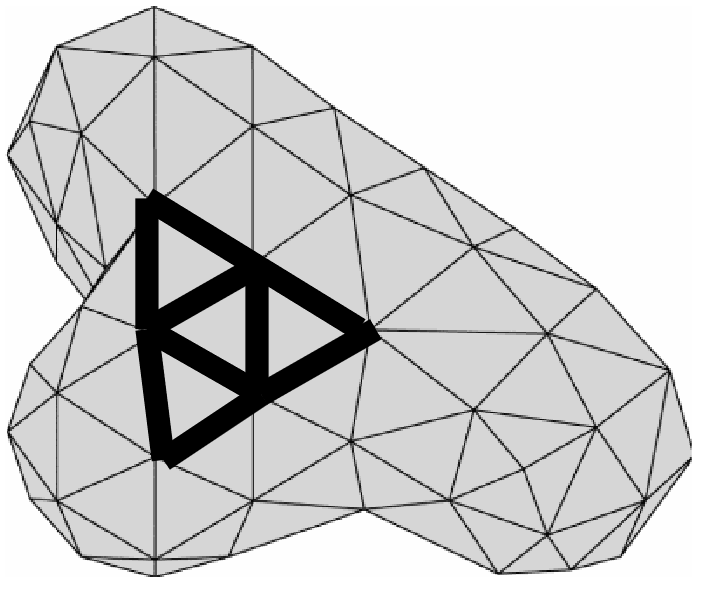
\includegraphics[width=0.3\columnwidth]{assets/loop-subdivision.png}
}
\makecell {
  \textbf{Butterfly} \\
  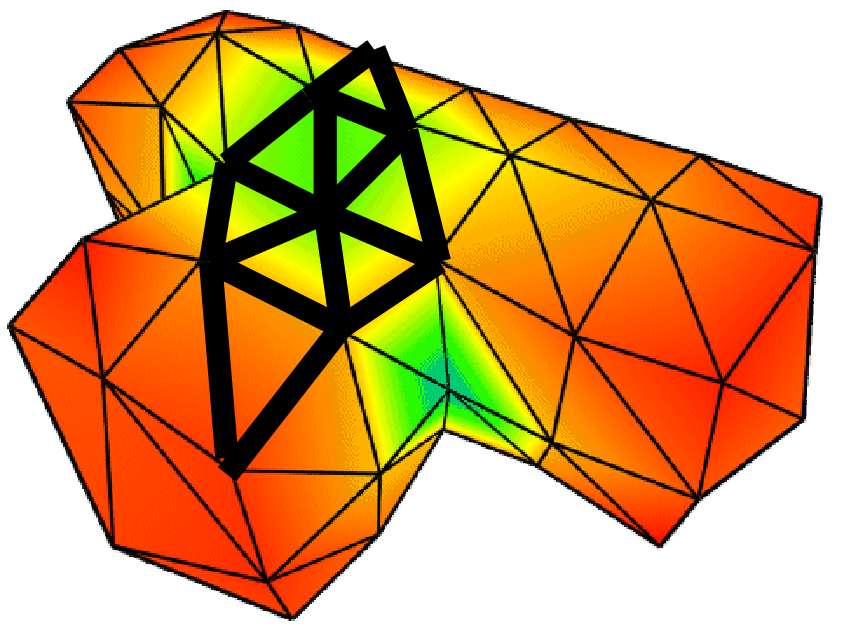
\includegraphics[width=0.3\columnwidth]{assets/butterfly.png}
}
\section{Visibility and Shadows}

\begin{algorithm}[Painter's algorithm]
  Render from furthest to nearest.

  \textit{Problems}:
  \begin{itemize*}
    \item cyclic overlaps
    \item intersections
  \end{itemize*}
\end{algorithm}

\begin{algorithm}[Z-Buffering]
  Store depth to nearest object per pixel.

  \begin{enumerate}
    \item Initialize all \(z\) values to \(\infty\)
    \item For each polygon: If new value smaller, replace!
  \end{enumerate}

  \textit{Problems}:
  \begin{itemize*}
    \item limited resolution
    \item resolution is non-linear
  \end{itemize*}
\end{algorithm}

\subsection{Shadows}

\begin{definition}[Planar Shadows]
  Draw projection on the ground.

  \textit{Limitations}:
  No self shadows or on other objects.
  Problems with curved surfaces.
\end{definition}

\begin{definition}[Projective texture shadows]
  Separate obstacle and receiver. Compute b/w image from light and use as projective texture.

  \textit{Limitations}:
  Need to specify obstacle \& receiver.
  No self-shadows.
\end{definition}

\begin{algorithm}[Shadow Maps]
  Compute depths from light \(d(x_L)\) and camera.
  For each pixel in camera plane:
  \begin{enumerate}
    \item Compute point in world coordinates
    \item Project onto light plane \(z_L\)
    \item If \(d(x_L) < z_L\), then \(x\) is in shadow.
  \end{enumerate}

  Add bias for stability (\(d(x_L) + b < z_L\)).

  A point to shadow can be outside the FoV of shadow map, thus use cubical shadow map or spot lights.

  Should \textbf{not} filter depth, but take weighted average.
\end{algorithm}

\begin{algorithm}[Shadow Volumes]
  Explicitly represent the volume of space in shadow. If polygon in volume, it is in shadow.

  \begin{enumerate}
    \item Shoot a ray from the camera
    \item ++/-- counter each time volume is intersected.
    \item if counter \(> 0\), then primitive is in shadow
  \end{enumerate}

  Use silhouette edges only!

  \textit{Limitations}:
  Lots of geometry.
  Expensive to rasterize long skinny triangles.
  Object must be watertight
  Rasterization of polygons sharing an edge must not overlap and not have gap.
\end{algorithm}

\section{Ray Tracing}

\begin{definition}[Ray Casting]
  Shoot ray through from the camera through the pixels and in first intersection, evaluate the illumination model.
\end{definition}

\begin{definition}[Forward Raytracing]
  Rays from light source (not efficient).
\end{definition}

\begin{definition}[Backward Raytracing]
  Shoot rays from the camera.
\end{definition}

\begin{definition}[The Pipeline]
  \begin{enumerate}
    \item \textit{Ray Generation}: Shoot ray from origin.
    \item \textit{Intersection}: Calculate first intersection. Calculate illumination at that point by recursion (either reflect or refract).
    \item \textit{Shading}: Shoot ray from intersection to directly to light source. Intersection \(\implies\) Point in shadow.
  \end{enumerate}
\end{definition}

\begin{definition}[Supersampling]
  Shoot multiple rays to remove aliasing.
\end{definition}

\subsection{The Math}

\begin{definition}[Ray Equation]
  \(r(t) = \vec{o} + t \vec{d}\) with \(\vec{o}\) origin and \(\vec{d}\) direction.
\end{definition}

\begin{definition}[Sphere Intersection]
  \(||x - \text{center}||^2 - \text{radius}^2 = 0\), then we plug in the ray equation into \(x\).
\end{definition}

\begin{definition}[Triangle]
  Use barycentric coordinates: \(x = s_1 p_1 + s_2 p_2 + s_3 p_3\) for the triangle \(p_1p_2p_3\).
  Intersect with triangle's plane:
  \[(\vec{o} + t\vec{d} - p_1) \cdot \vec{n} = 0 \quad t = \frac{(\vec{o} - p_1) \cdot n}{\vec{d} \cdot n} \quad n = (p_2 - p_1) \times (p_3 - p_1)\]
  We compute \(s_i\), then test: \(s_1 + s_2 + s_3 = 0 \ \land \ s_i \in [0,1]\)
\end{definition}

\subsection{Shading}
Physical shading too costly, thus simple assumptions:
\begin{itemize}
  \item \textit{Surface Reflectance}: Diffuse, specular, ambient, transp.
  \item \textit{Shadows}: Shadow rays as described above
\end{itemize}

\begin{definition}[Refraction]
  Add probability to refract from turned normal.
\end{definition}

\begin{definition}[Multiple lights]
  Iterate shadow rays over multiple lights.
\end{definition}

\begin{definition}[Area lights]
  Add soft shadows with area lights.
\end{definition}

\begin{definition}[Motion Blur]
  Sample objects and intersect in time.
\end{definition}

\begin{definition}[Depth of field]
  Add virtual "lens" with focal length.
\end{definition}



% Math stuff
\clearpage
\section{Quick Maths}

\subsection{Quaternions}

Properties:
\begin{align*}
  i^2=j^2=k^2 = -1, \quad ijk = -1, \quad ij=k, \quad ji=-k \\ \quad jk=i, \quad kj = -i, \quad ki = j, \quad ik = -j \\
  \lVert q \rVert = \sqrt{a^2+b^2+c^2+d^2},\\ \text{where } q = a + \left[\begin{smallmatrix} b & c & d \end{smallmatrix}\right] \left[\begin{smallmatrix} i \\ j \\ k \end{smallmatrix}\right] = a + v \text{ ,v not vector!} \\
  \overline{z} = a - bi - cj - dk, \quad z^{-1} = \frac{\overline{z}}{\lVert z \rVert}
\end{align*}

\subsection{Rotation with quaternions}

Rotate \( p = \left[\begin{smallmatrix} x & y & z \end{smallmatrix}\right] \) around axis \( u = \left[\begin{smallmatrix} u_{1} & u_{2} & u_{3} \end{smallmatrix}\right] \) by angle \( \theta  \).
\begin{enumerate}
  \item Convert \( p \) to quaternion \( p_Q = xi + yj + zk \)
  \item Convert u to quaternion \( q'' = u_{1}i+u_{2}j+u_{3}k \) and \\ normalize \( q'' \) to \( q' = \sfrac{q''}{\lVert q'' \rVert} \)
  \item Rotation quaternion \( q = \cos (\theta /2) + \sin (\theta /2) q' \) \\ and \( q^{-1} = \cos (\theta /2) - \sin (\theta /2) q' \)
  \item Rotated point \( p' = q p q^{-1} \)
  \item Convert \( p' \) back to cartesian
\end{enumerate}
Half angle because rotate twice, one from left, and once from right (using inverse). This is done to undo the scaling and use inverse to rotate further in the same direction (multiplied from the other side), otherwise, also rotation is undone.

\subsection{Interpolation}

\begin{definition}[Bilinear Interpolation]
  \(f(x,y) = (1-a)(1-b) \cdot f(i,j) + a(1-b) \cdot f(i+1,j) + ab \cdot f(i+1, j+1) + (1-a)b \cdot f(i,j+1)\)
\end{definition}

\subsection{Trigonometry}
\(\sin(x) = \frac{e^{ix} - e^{-ix}}{2i} \quad \cos(x) = \frac{e^{ix} + e^{-ix}}{2}\) \\
\(\sin(2x) = 2\sin(x)\cos(x) \\ \cos(2x) = \cos^2(x) - \sin^2(x) \\ \sin(x+y) = \sin(x)\cos(y) + \cos(x)\sin(y) \\ \cos(x+y) = \cos(x)\cos(y) + \sin(x)\cos(y) \\ \sin^2(x) + \cos^2(x) = 1\)

\begin{center}
  \begin{tabular}{|c|c|c|c|c|c|c|}
  \hline
  & \(0\) & \(\pi/6\) & \(\pi/4\) & \(\pi/3\) & \(\pi/2\) & \(\pi\) \\
  \hline
  \textbf{Sine} & \(0\) & \(\frac{1}{2}\) & \(\frac{\sqrt{2}}{2}\) & \(\frac{\sqrt{3}}{2}\) & \(1\) & \(0\) \\
  \hline
  \textbf{Cosine} & \(1\) & \(\frac{\sqrt{3}}{2}\) & \(\frac{\sqrt{2}}{2}\) & \(\frac{1}{2}\) & \(0\) & \(-1\) \\
  \hline
  \end{tabular}
\end{center}

\subsection{Lucas Kanade Levels}

\textbf{Given}: \(\text{FPS}[\sfrac{f}{s}]\), \(v[\sfrac{m}{s}] = \frac{1}{3,6} \cdot (v^k[\sfrac{km}{h}])\), \(R[\sfrac{px}{m}]\).

\begin{enumerate}
  \item Calculate pixel per frame: \(\text{PPF}[\sfrac{px}{f}] = \frac{v[\sfrac{m}{s}] \cdot R[\frac{px}{m}]}{\text{FPS}[\sfrac{f}{s}]}\)
  \item Calculate levels: \(1 + \lceil \log_2 \text{PPF} \rceil\)
\end{enumerate}

\subsection{PCA Proofs}

\begin{definition}[Optimal Energy Concentration of KLT]
  Consider truncated coefficient vector \(\vec{b} = I_J \vec{c}\) {\color{gray}(\(I_J\): ID matrix with first \(J\) columns)} Energy in first \(J\) coefficients for an arbitrary transform \(A\):

  \(E = \text{Tr}(R_{bb}) = \text{Tr}(I_J R_{cc} I_{J}) = \text{Tr}(I_J A R_{ff} A^H I_J) = \sum_{k = 0}^{J - 1} a_k^T R_{ff} a_k^*\) where \(a_k^T\) is \(k\)-th row of \(A\).
  Lagrangian cost function to enforce unit-length basis vectors:
  \(L = E + \sum_{k = 0}^{J - 1} \lambda_k (1 - a_k^T a_k^*) =\) \\
  \( \sum_{k = 0}^{J - 1} a_k^T R_{ff} a_k^* + \sum_{k = 0}^{J - 1} \lambda_k (1 - a_k^T a_k^*)\)

  Differentiating \(L\) with respect to \(a_j\): \(R_{ff} a_j^* = \lambda_i a_j^* \quad \forall_j < J\) {\color{gray}{necessary condition}}
\end{definition}

\pagebreak

\begin{definition}[Energy Concentration of first principal component]
  The one corresponding to the largest eigenvalue.
  \[
  \begin{aligned}
  E_k & =\sum_i\left[\left(\sum_j z_{i, j} \boldsymbol{u}_{\boldsymbol{j}}+\overline{\boldsymbol{x}}\right)-\left(z_{i, k} \boldsymbol{u}_{\boldsymbol{k}}+\overline{\boldsymbol{x}}\right)\right]^2 \\
  & =\sum_i\left[\sum_{j \neq k} z_{i, j} \boldsymbol{u}_{\boldsymbol{j}}\right]^2 \\
  & \left.=\sum_i \sum_{j \neq k} z_{i, j}^2(\text { eigenvectors are linearly independent })\right) \\
  & =\sum_i \sum_{j \neq k}\left[\boldsymbol{u}_{\boldsymbol{j}} \cdot\left(\boldsymbol{x}_{\boldsymbol{i}}-\overline{\boldsymbol{x}}\right)^T\right]^2 \\
  & =\sum_i \sum_{j \neq k} \boldsymbol{u}_{\boldsymbol{j}} \cdot\left(\boldsymbol{x}_{\boldsymbol{i}}-\overline{\boldsymbol{x}}\right)^T \cdot\left(\boldsymbol{x}_{\boldsymbol{i}}-\overline{\boldsymbol{x}}\right) \cdot \boldsymbol{u}_{\boldsymbol{j}}{ }^T \\
  & =\sum_{j \neq k} \boldsymbol{u}_{\boldsymbol{j}} \boldsymbol{\Sigma} \boldsymbol{u}_{\boldsymbol{j}}{ }^T=\sum_{j \neq k} \lambda_j
  \end{aligned}
  \]
  As shown, \(E_k\) is the sum of all eigenvalues except \(\lambda_k\). Therefore, \(E_k\) is minimized if \(\lambda_k\) is the largest eigenvalue.
\end{definition}

\begin{definition}[PCA Cost]
  Consider \(K\) eigenfaces, \(N\) images, \(L \times W\) dimensions of images.
  \begin{itemize*}
    \item \textit{Mean image}: \(L \times W\)
    \item \textit{Eigenfaces}: \(K \times L \times W\)
    \item \textit{Compressed images}: \(N \times K\)
    \item \textit{save space}: \(K < \frac{(N - 1) \times L \times W}{N + L \times W}\)
  \end{itemize*}
\end{definition}



\end{document}
